\documentclass{article}

\PassOptionsToPackage{numbers, compress}{natbib}
\usepackage{neurips_2026}

\usepackage[utf8]{inputenc}
\usepackage[T1]{fontenc}
\usepackage{hyperref}
\usepackage{url}
\usepackage{booktabs}
\usepackage{amsfonts}
\usepackage{amsmath}
\usepackage{amssymb}
\usepackage{amsthm}
\usepackage{nicefrac}
\usepackage{microtype}
\usepackage{xcolor}
\usepackage{graphicx}
\usepackage{multirow}
\usepackage{tikz}
\usetikzlibrary{arrows.meta}
\usepackage{enumitem}
\setlist{itemsep=1pt,topsep=3pt,parsep=0pt}

\newtheorem{proposition}{Proposition}
\newtheorem{remark}{Remark}
\newcommand{\R}{\mathbb{R}}
\newcommand{\N}{\mathcal{N}}
\newcommand{\D}{\mathcal{D}}

\newcommand{\AblCav}{$+$0.026}
\newcommand{\AblCavabs}{0.026}
\newcommand{\AblCavci}{[$+$0.022, $+$0.029]}
\newcommand{\AblLift}{$+$0.134}
\newcommand{\AblLiftabs}{0.134}
\newcommand{\AblLiftci}{[$+$0.120, $+$0.148]}
\newcommand{\AblliftOnestaticvsfa}{$+$0.054}
\newcommand{\AblliftOnestaticvsfaabs}{0.054}
\newcommand{\AblliftOnevsfa}{$+$0.080}
\newcommand{\AblliftOnevsfaabs}{0.080}
\newcommand{\AblliftTwovsfa}{$+$0.079}
\newcommand{\AblliftTwovsfaabs}{0.079}
\newcommand{\AblliftZerovsfa}{$-$0.054}
\newcommand{\AblliftZerovsfaabs}{0.054}
\newcommand{\Ablrepocavityfreshvsfa}{$-$0.159}
\newcommand{\Ablrepocavityfreshvsfaabs}{0.159}
\newcommand{\CalanchormlpFcov}{0.902}
\newcommand{\CalanchormlpFcrps}{0.162}
\newcommand{\CalanchormlpFrmse}{0.309}
\newcommand{\CalblrccBcov}{0.861}
\newcommand{\CalblrccBcrps}{0.182}
\newcommand{\CalblrccBrmse}{0.374}
\newcommand{\CalblrccFcov}{0.866}
\newcommand{\CalblrccFcrps}{0.174}
\newcommand{\CalblrccFrmse}{0.327}
\newcommand{\CalemgaussBcov}{0.807}
\newcommand{\CalemgaussBcrps}{0.207}
\newcommand{\CalemgaussBrmse}{0.423}
\newcommand{\CalemgaussFcov}{0.860}
\newcommand{\CalemgaussFcrps}{0.170}
\newcommand{\CalemgaussFrmse}{0.318}
\newcommand{\CalfaOneBcov}{0.824}
\newcommand{\CalfaOneBcrps}{0.189}
\newcommand{\CalfaOneBrmse}{0.379}
\newcommand{\CalfaOneFcov}{0.873}
\newcommand{\CalfaOneFcrps}{0.168}
\newcommand{\CalfaOneFrmse}{0.316}
\newcommand{\CalliftOneBcov}{0.914}
\newcommand{\CalliftOneBcrps}{0.171}
\newcommand{\CalliftOneBrmse}{0.357}
\newcommand{\CalliftOneFcov}{0.901}
\newcommand{\CalliftOneFcrps}{0.160}
\newcommand{\CalliftOneFrmse}{0.305}
\newcommand{\CalpfnBcov}{0.914}
\newcommand{\CalpfnBcrps}{0.158}
\newcommand{\CalpfnBrmse}{0.341}
\newcommand{\CalpfnFcov}{0.902}
\newcommand{\CalpfnFcrps}{0.165}
\newcommand{\CalpfnFrmse}{0.314}
\newcommand{\Computetrainratio}{14}
\newcommand{\FTbeijinggapqQFour}{0.01}
\newcommand{\FTbeijinggapqQOne}{0.15}
\newcommand{\FTbeijinggapqQThree}{0.15}
\newcommand{\FTbeijinggapqQTwo}{0.16}
\newcommand{\FTbeijingliftgain}{0.62}
\newcommand{\FTbeijingpfnbetterpct}{89}
\newcommand{\FTbeijingpfngain}{0.87}
\newcommand{\FTbeijingtraingap}{0.19}
\newcommand{\Fanchormlpka}{$-$0.236}
\newcommand{\Fanchormlpkaabs}{0.236}
\newcommand{\Fanchormlpkb}{$-$0.087}
\newcommand{\Fanchormlpkbabs}{0.087}
\newcommand{\Fanchormlpkc}{0.114}
\newcommand{\Fanchormlpkd}{0.397}
\newcommand{\Fblrccka}{0.111}
\newcommand{\Fblrcckb}{0.091}
\newcommand{\Fblrcckc}{0.214}
\newcommand{\Fblrcckd}{0.450}
\newcommand{\Fbopka}{$-$0.334}
\newcommand{\Fbopkaabs}{0.334}
\newcommand{\Fbopkb}{$-$0.174}
\newcommand{\Fbopkbabs}{0.174}
\newcommand{\Fbopkc}{0.039}
\newcommand{\Fbopkd}{0.337}
\newcommand{\Femgausska}{$-$0.048}
\newcommand{\Femgausskaabs}{0.048}
\newcommand{\Femgausskb}{0.037}
\newcommand{\Femgausskc}{0.195}
\newcommand{\Femgausskd}{0.441}
\newcommand{\FfaOneka}{$-$0.152}
\newcommand{\FfaOnekaabs}{0.152}
\newcommand{\FfaOnekb}{$-$0.011}
\newcommand{\FfaOnekbabs}{0.011}
\newcommand{\FfaOnekc}{0.177}
\newcommand{\FfaOnekd}{0.439}
\newcommand{\Fgpkc}{0.416}
\newcommand{\Flctka}{$-$0.265}
\newcommand{\Flctkaabs}{0.265}
\newcommand{\Flctkb}{$-$0.112}
\newcommand{\Flctkbabs}{0.112}
\newcommand{\Flctkc}{0.095}
\newcommand{\Flctkd}{0.387}
\newcommand{\FliftOneka}{$-$0.265}
\newcommand{\FliftOnekaabs}{0.265}
\newcommand{\FliftOnekb}{$-$0.112}
\newcommand{\FliftOnekbabs}{0.112}
\newcommand{\FliftOnekc}{0.097}
\newcommand{\FliftOnekd}{0.395}
\newcommand{\Fnlfaka}{$-$0.173}
\newcommand{\Fnlfakaabs}{0.173}
\newcommand{\Fnlfakb}{$-$0.036}
\newcommand{\Fnlfakbabs}{0.036}
\newcommand{\Fnlfakc}{0.151}
\newcommand{\Fnlfakd}{0.417}
\newcommand{\Foracleka}{$-$0.419}
\newcommand{\Foraclekaabs}{0.419}
\newcommand{\Foraclekb}{$-$0.250}
\newcommand{\Foraclekbabs}{0.250}
\newcommand{\Foraclekc}{$-$0.026}
\newcommand{\Foraclekcabs}{0.026}
\newcommand{\Foraclekd}{0.287}
\newcommand{\Fpfnallka}{$-$0.237}
\newcommand{\Fpfnallkaabs}{0.237}
\newcommand{\Fpfnallkb}{$-$0.076}
\newcommand{\Fpfnallkbabs}{0.076}
\newcommand{\Fpfnallkc}{0.132}
\newcommand{\Fpfnallkd}{0.411}
\newcommand{\Fpfnka}{$-$0.246}
\newcommand{\Fpfnkaabs}{0.246}
\newcommand{\Fpfnkb}{$-$0.084}
\newcommand{\Fpfnkbabs}{0.084}
\newcommand{\Fpfnkc}{0.131}
\newcommand{\Fpfnkd}{0.424}
\newcommand{\Frepocavityfreshka}{0.055}
\newcommand{\Frepocavityfreshkb}{0.178}
\newcommand{\Frepocavityfreshkc}{0.336}
\newcommand{\Frepocavityfreshkd}{0.555}
\newcommand{\Fridgeccka}{0.026}
\newcommand{\Fridgecckb}{0.078}
\newcommand{\Fridgecckc}{0.216}
\newcommand{\Fridgecckd}{0.451}
\newcommand{\Fridgerepoka}{0.198}
\newcommand{\Fridgerepokb}{0.280}
\newcommand{\Fridgerepokc}{0.399}
\newcommand{\Fridgerepokd}{0.582}
\newcommand{\Gapanchormlp}{46}
\newcommand{\Gaplct}{59}
\newcommand{\GapliftOne}{58}
\newcommand{\Gapnlfa}{19}
\newcommand{\Gappfn}{34}
\newcommand{\Gappfnall}{33}
\newcommand{\MainkKOneliftvsmlp}{$+$0.024}
\newcommand{\MainkKOneliftvsmlpabs}{0.024}
\newcommand{\MainkKOneliftvsmlpci}{[$+$0.019, $+$0.030]}
\newcommand{\MainkKOneliftvspfn}{$+$0.028}
\newcommand{\MainkKOneliftvspfnabs}{0.028}
\newcommand{\MainkKOneliftvspfnall}{$+$0.036}
\newcommand{\MainkKOneliftvspfnallabs}{0.036}
\newcommand{\MainkKOneliftvspfnallci}{[$+$0.028, $+$0.044]}
\newcommand{\MainkKOneliftvspfnci}{[$+$0.020, $+$0.035]}
\newcommand{\MainkKThreeliftvsmlp}{$+$0.002}
\newcommand{\MainkKThreeliftvsmlpabs}{0.002}
\newcommand{\MainkKThreeliftvsmlpci}{[$-$0.001, $+$0.005]}
\newcommand{\MainkKThreeliftvspfn}{$+$0.029}
\newcommand{\MainkKThreeliftvspfnabs}{0.029}
\newcommand{\MainkKThreeliftvspfnall}{$+$0.017}
\newcommand{\MainkKThreeliftvspfnallabs}{0.017}
\newcommand{\MainkKThreeliftvspfnallci}{[$+$0.012, $+$0.022]}
\newcommand{\MainkKThreeliftvspfnci}{[$+$0.024, $+$0.035]}
\newcommand{\MainkKTwoliftvsmlp}{$+$0.016}
\newcommand{\MainkKTwoliftvsmlpabs}{0.016}
\newcommand{\MainkKTwoliftvsmlpci}{[$+$0.013, $+$0.020]}
\newcommand{\MainkKTwoliftvspfn}{$+$0.033}
\newcommand{\MainkKTwoliftvspfnabs}{0.033}
\newcommand{\MainkKTwoliftvspfnall}{$+$0.035}
\newcommand{\MainkKTwoliftvspfnallabs}{0.035}
\newcommand{\MainkKTwoliftvspfnallci}{[$+$0.028, $+$0.042]}
\newcommand{\MainkKTwoliftvspfnci}{[$+$0.027, $+$0.040]}
\newcommand{\MainkKZeroliftvsmlp}{$+$0.030}
\newcommand{\MainkKZeroliftvsmlpabs}{0.030}
\newcommand{\MainkKZeroliftvsmlpci}{[$+$0.022, $+$0.037]}
\newcommand{\MainkKZeroliftvspfn}{$+$0.020}
\newcommand{\MainkKZeroliftvspfnabs}{0.020}
\newcommand{\MainkKZeroliftvspfnall}{$+$0.028}
\newcommand{\MainkKZeroliftvspfnallabs}{0.028}
\newcommand{\MainkKZeroliftvspfnallci}{[$+$0.017, $+$0.039]}
\newcommand{\MainkKZeroliftvspfnci}{[$+$0.009, $+$0.030]}
\newcommand{\RairqcoeTwopfnvsblr}{$+$0.268}
\newcommand{\RairqcoeTwopfnvsblrabs}{0.268}
\newcommand{\RairqcoeTwopfnvsblrci}{[$+$0.076, $+$0.459]}
\newcommand{\RairqcoeTwovalblr}{0.216}
\newcommand{\RairqcoeTwovalem}{0.085}
\newcommand{\RairqcoeTwovalfa}{0.116}
\newcommand{\RairqcoeTwovalftlift}{0.008}
\newcommand{\RairqcoeTwovalftpfn}{$-$0.052}
\newcommand{\RairqcoeTwovalftpfnabs}{0.052}
\newcommand{\RairqcoeTwovalgp}{0.503}
\newcommand{\RairqcoeTwovalknn}{0.353}
\newcommand{\RairqcoeTwovalnlfa}{0.091}
\newcommand{\RairqcoeTwovalzslift}{0.129}
\newcommand{\RairqcoeTwovalzspfn}{0.081}
\newcommand{\RairqcoeTwovsblr}{$+$0.208}
\newcommand{\RairqcoeTwovsblrabs}{0.208}
\newcommand{\RairqcoeTwovsblrci}{[$+$0.036, $+$0.379]}
\newcommand{\RairqcoeTwovsem}{$+$0.077}
\newcommand{\RairqcoeTwovsemabs}{0.077}
\newcommand{\RairqcoeTwovsemci}{[$-$0.013, $+$0.166]}
\newcommand{\RairqcoeTwovsfa}{$+$0.107}
\newcommand{\RairqcoeTwovsfaabs}{0.107}
\newcommand{\RairqcoeTwovsfaci}{[$+$0.015, $+$0.200]}
\newcommand{\RairqcoeTwovsmlp}{$+$0.102}
\newcommand{\RairqcoeTwovsmlpabs}{0.102}
\newcommand{\RairqcoeTwovsmlpci}{[$+$0.007, $+$0.197]}
\newcommand{\RairqcoeTwovsnopre}{$-$0.015}
\newcommand{\RairqcoeTwovsnopreabs}{0.015}
\newcommand{\RairqcoeTwovsnopreci}{[$-$0.044, $+$0.014]}
\newcommand{\RairqcoeTwovspfn}{$-$0.060}
\newcommand{\RairqcoeTwovspfnabs}{0.060}
\newcommand{\RairqcoeTwovspfnci}{[$-$0.106, $-$0.014]}
\newcommand{\RairqcoeTwovsstatic}{$-$0.037}
\newcommand{\RairqcoeTwovsstaticabs}{0.037}
\newcommand{\RairqcoeTwovsstaticci}{[$-$0.078, $+$0.004]}
\newcommand{\RairqcoeTwozsliftvspfn}{$-$0.048}
\newcommand{\RairqcoeTwozsliftvspfnabs}{0.048}
\newcommand{\RairqcoeTwozsliftvspfnci}{[$-$0.084, $-$0.012]}
\newcommand{\RairqcoeZeropfnvsblr}{$+$1.200}
\newcommand{\RairqcoeZeropfnvsblrabs}{1.200}
\newcommand{\RairqcoeZeropfnvsblrci}{[$-$0.155, $+$2.555]}
\newcommand{\RairqcoeZerovalblr}{1.037}
\newcommand{\RairqcoeZerovalem}{0.074}
\newcommand{\RairqcoeZerovalfa}{0.052}
\newcommand{\RairqcoeZerovalftlift}{$-$0.040}
\newcommand{\RairqcoeZerovalftliftabs}{0.040}
\newcommand{\RairqcoeZerovalftpfn}{$-$0.163}
\newcommand{\RairqcoeZerovalftpfnabs}{0.163}
\newcommand{\RairqcoeZerovalgp}{3.364}
\newcommand{\RairqcoeZerovalknn}{0.571}
\newcommand{\RairqcoeZerovalnlfa}{0.144}
\newcommand{\RairqcoeZerovalzslift}{0.044}
\newcommand{\RairqcoeZerovalzspfn}{$-$0.017}
\newcommand{\RairqcoeZerovalzspfnabs}{0.017}
\newcommand{\RairqcoeZerovsblr}{$+$1.077}
\newcommand{\RairqcoeZerovsblrabs}{1.077}
\newcommand{\RairqcoeZerovsblrci}{[$-$0.278, $+$2.432]}
\newcommand{\RairqcoeZerovsem}{$+$0.113}
\newcommand{\RairqcoeZerovsemabs}{0.113}
\newcommand{\RairqcoeZerovsemci}{[$-$0.061, $+$0.288]}
\newcommand{\RairqcoeZerovsfa}{$+$0.092}
\newcommand{\RairqcoeZerovsfaabs}{0.092}
\newcommand{\RairqcoeZerovsfaci}{[$-$0.034, $+$0.217]}
\newcommand{\RairqcoeZerovsmlp}{$+$0.064}
\newcommand{\RairqcoeZerovsmlpabs}{0.064}
\newcommand{\RairqcoeZerovsmlpci}{[$-$0.063, $+$0.192]}
\newcommand{\RairqcoeZerovsnopre}{$+$0.039}
\newcommand{\RairqcoeZerovsnopreabs}{0.039}
\newcommand{\RairqcoeZerovsnopreci}{[$-$0.029, $+$0.106]}
\newcommand{\RairqcoeZerovspfn}{$-$0.124}
\newcommand{\RairqcoeZerovspfnabs}{0.124}
\newcommand{\RairqcoeZerovspfnci}{[$-$0.202, $-$0.045]}
\newcommand{\RairqcoeZerovsstatic}{$-$0.046}
\newcommand{\RairqcoeZerovsstaticabs}{0.046}
\newcommand{\RairqcoeZerovsstaticci}{[$-$0.131, $+$0.038]}
\newcommand{\RairqcoeZerozsliftvspfn}{$-$0.061}
\newcommand{\RairqcoeZerozsliftvspfnabs}{0.061}
\newcommand{\RairqcoeZerozsliftvspfnci}{[$-$0.130, $+$0.008]}
\newcommand{\Rairqcoepisodes}{23}
\newcommand{\Rairqconatmiss}{0.0}
\newcommand{\RairqnoTwoeTwopfnvsblr}{$+$0.203}
\newcommand{\RairqnoTwoeTwopfnvsblrabs}{0.203}
\newcommand{\RairqnoTwoeTwopfnvsblrci}{[$+$0.111, $+$0.295]}
\newcommand{\RairqnoTwoeTwovalblr}{$-$0.178}
\newcommand{\RairqnoTwoeTwovalblrabs}{0.178}
\newcommand{\RairqnoTwoeTwovalem}{$-$0.175}
\newcommand{\RairqnoTwoeTwovalemabs}{0.175}
\newcommand{\RairqnoTwoeTwovalfa}{$-$0.155}
\newcommand{\RairqnoTwoeTwovalfaabs}{0.155}
\newcommand{\RairqnoTwoeTwovalftlift}{$-$0.337}
\newcommand{\RairqnoTwoeTwovalftliftabs}{0.337}
\newcommand{\RairqnoTwoeTwovalftpfn}{$-$0.381}
\newcommand{\RairqnoTwoeTwovalftpfnabs}{0.381}
\newcommand{\RairqnoTwoeTwovalgp}{$-$0.198}
\newcommand{\RairqnoTwoeTwovalgpabs}{0.198}
\newcommand{\RairqnoTwoeTwovalknn}{$-$0.063}
\newcommand{\RairqnoTwoeTwovalknnabs}{0.063}
\newcommand{\RairqnoTwoeTwovalnlfa}{$-$0.142}
\newcommand{\RairqnoTwoeTwovalnlfaabs}{0.142}
\newcommand{\RairqnoTwoeTwovalzslift}{$-$0.233}
\newcommand{\RairqnoTwoeTwovalzsliftabs}{0.233}
\newcommand{\RairqnoTwoeTwovalzspfn}{$-$0.231}
\newcommand{\RairqnoTwoeTwovalzspfnabs}{0.231}
\newcommand{\RairqnoTwoeTwovsblr}{$+$0.159}
\newcommand{\RairqnoTwoeTwovsblrabs}{0.159}
\newcommand{\RairqnoTwoeTwovsblrci}{[$+$0.073, $+$0.245]}
\newcommand{\RairqnoTwoeTwovsem}{$+$0.162}
\newcommand{\RairqnoTwoeTwovsemabs}{0.162}
\newcommand{\RairqnoTwoeTwovsemci}{[$+$0.046, $+$0.278]}
\newcommand{\RairqnoTwoeTwovsfa}{$+$0.181}
\newcommand{\RairqnoTwoeTwovsfaabs}{0.181}
\newcommand{\RairqnoTwoeTwovsfaci}{[$+$0.076, $+$0.287]}
\newcommand{\RairqnoTwoeTwovsmlp}{$+$0.190}
\newcommand{\RairqnoTwoeTwovsmlpabs}{0.190}
\newcommand{\RairqnoTwoeTwovsmlpci}{[$+$0.116, $+$0.264]}
\newcommand{\RairqnoTwoeTwovsnopre}{$+$0.021}
\newcommand{\RairqnoTwoeTwovsnopreabs}{0.021}
\newcommand{\RairqnoTwoeTwovsnopreci}{[$+$0.005, $+$0.036]}
\newcommand{\RairqnoTwoeTwovspfn}{$-$0.044}
\newcommand{\RairqnoTwoeTwovspfnabs}{0.044}
\newcommand{\RairqnoTwoeTwovspfnci}{[$-$0.074, $-$0.014]}
\newcommand{\RairqnoTwoeTwovsstatic}{$+$0.005}
\newcommand{\RairqnoTwoeTwovsstaticabs}{0.005}
\newcommand{\RairqnoTwoeTwovsstaticci}{[$-$0.013, $+$0.023]}
\newcommand{\RairqnoTwoeTwozsliftvspfn}{$+$0.003}
\newcommand{\RairqnoTwoeTwozsliftvspfnabs}{0.003}
\newcommand{\RairqnoTwoeTwozsliftvspfnci}{[$-$0.045, $+$0.050]}
\newcommand{\RairqnoTwoeZeropfnvsblr}{$+$0.430}
\newcommand{\RairqnoTwoeZeropfnvsblrabs}{0.430}
\newcommand{\RairqnoTwoeZeropfnvsblrci}{[$+$0.252, $+$0.607]}
\newcommand{\RairqnoTwoeZerovalblr}{$-$0.055}
\newcommand{\RairqnoTwoeZerovalblrabs}{0.055}
\newcommand{\RairqnoTwoeZerovalem}{$-$0.237}
\newcommand{\RairqnoTwoeZerovalemabs}{0.237}
\newcommand{\RairqnoTwoeZerovalfa}{$-$0.196}
\newcommand{\RairqnoTwoeZerovalfaabs}{0.196}
\newcommand{\RairqnoTwoeZerovalftlift}{$-$0.412}
\newcommand{\RairqnoTwoeZerovalftliftabs}{0.412}
\newcommand{\RairqnoTwoeZerovalftpfn}{$-$0.485}
\newcommand{\RairqnoTwoeZerovalftpfnabs}{0.485}
\newcommand{\RairqnoTwoeZerovalgp}{25.217}
\newcommand{\RairqnoTwoeZerovalknn}{$-$0.010}
\newcommand{\RairqnoTwoeZerovalknnabs}{0.010}
\newcommand{\RairqnoTwoeZerovalnlfa}{$-$0.090}
\newcommand{\RairqnoTwoeZerovalnlfaabs}{0.090}
\newcommand{\RairqnoTwoeZerovalzslift}{$-$0.350}
\newcommand{\RairqnoTwoeZerovalzsliftabs}{0.350}
\newcommand{\RairqnoTwoeZerovalzspfn}{$-$0.360}
\newcommand{\RairqnoTwoeZerovalzspfnabs}{0.360}
\newcommand{\RairqnoTwoeZerovsblr}{$+$0.357}
\newcommand{\RairqnoTwoeZerovsblrabs}{0.357}
\newcommand{\RairqnoTwoeZerovsblrci}{[$+$0.184, $+$0.530]}
\newcommand{\RairqnoTwoeZerovsem}{$+$0.175}
\newcommand{\RairqnoTwoeZerovsemabs}{0.175}
\newcommand{\RairqnoTwoeZerovsemci}{[$-$0.010, $+$0.360]}
\newcommand{\RairqnoTwoeZerovsfa}{$+$0.216}
\newcommand{\RairqnoTwoeZerovsfaabs}{0.216}
\newcommand{\RairqnoTwoeZerovsfaci}{[$+$0.027, $+$0.405]}
\newcommand{\RairqnoTwoeZerovsmlp}{$+$0.166}
\newcommand{\RairqnoTwoeZerovsmlpabs}{0.166}
\newcommand{\RairqnoTwoeZerovsmlpci}{[$+$0.039, $+$0.293]}
\newcommand{\RairqnoTwoeZerovsnopre}{$-$0.007}
\newcommand{\RairqnoTwoeZerovsnopreabs}{0.007}
\newcommand{\RairqnoTwoeZerovsnopreci}{[$-$0.046, $+$0.032]}
\newcommand{\RairqnoTwoeZerovspfn}{$-$0.072}
\newcommand{\RairqnoTwoeZerovspfnabs}{0.072}
\newcommand{\RairqnoTwoeZerovspfnci}{[$-$0.102, $-$0.042]}
\newcommand{\RairqnoTwoeZerovsstatic}{$-$0.010}
\newcommand{\RairqnoTwoeZerovsstaticabs}{0.010}
\newcommand{\RairqnoTwoeZerovsstaticci}{[$-$0.048, $+$0.027]}
\newcommand{\RairqnoTwoeZerozsliftvspfn}{$-$0.010}
\newcommand{\RairqnoTwoeZerozsliftvspfnabs}{0.010}
\newcommand{\RairqnoTwoeZerozsliftvspfnci}{[$-$0.067, $+$0.046]}
\newcommand{\RairqnoTwoepisodes}{23}
\newcommand{\RairqnoTwonatmiss}{0.0}
\newcommand{\RbeijingeSixpfnvsblr}{$+$0.206}
\newcommand{\RbeijingeSixpfnvsblrabs}{0.206}
\newcommand{\RbeijingeSixpfnvsblrci}{[$+$0.170, $+$0.241]}
\newcommand{\RbeijingeSixvalblr}{0.442}
\newcommand{\RbeijingeSixvalem}{0.569}
\newcommand{\RbeijingeSixvalfa}{0.562}
\newcommand{\RbeijingeSixvalftlift}{0.305}
\newcommand{\RbeijingeSixvalftpfn}{0.236}
\newcommand{\RbeijingeSixvalgp}{0.934}
\newcommand{\RbeijingeSixvalknn}{0.540}
\newcommand{\RbeijingeSixvalnlfa}{0.610}
\newcommand{\RbeijingeSixvalzslift}{0.561}
\newcommand{\RbeijingeSixvalzspfn}{0.687}
\newcommand{\RbeijingeSixvsblr}{$+$0.137}
\newcommand{\RbeijingeSixvsblrabs}{0.137}
\newcommand{\RbeijingeSixvsblrci}{[$+$0.104, $+$0.170]}
\newcommand{\RbeijingeSixvsem}{$+$0.265}
\newcommand{\RbeijingeSixvsemabs}{0.265}
\newcommand{\RbeijingeSixvsemci}{[$+$0.207, $+$0.322]}
\newcommand{\RbeijingeSixvsfa}{$+$0.258}
\newcommand{\RbeijingeSixvsfaabs}{0.258}
\newcommand{\RbeijingeSixvsfaci}{[$+$0.202, $+$0.314]}
\newcommand{\RbeijingeSixvsnopre}{$+$0.040}
\newcommand{\RbeijingeSixvsnopreabs}{0.040}
\newcommand{\RbeijingeSixvsnopreci}{[$+$0.032, $+$0.047]}
\newcommand{\RbeijingeSixvspfn}{$-$0.069}
\newcommand{\RbeijingeSixvspfnabs}{0.069}
\newcommand{\RbeijingeSixvspfnci}{[$-$0.080, $-$0.058]}
\newcommand{\RbeijingeSixvsstatic}{$+$0.044}
\newcommand{\RbeijingeSixvsstaticabs}{0.044}
\newcommand{\RbeijingeSixvsstaticci}{[$+$0.028, $+$0.060]}
\newcommand{\RbeijingeSixzsliftvspfn}{$+$0.127}
\newcommand{\RbeijingeSixzsliftvspfnabs}{0.127}
\newcommand{\RbeijingeSixzsliftvspfnci}{[$+$0.057, $+$0.197]}
\newcommand{\RbeijingeThreepfnvsblr}{$+$0.285}
\newcommand{\RbeijingeThreepfnvsblrabs}{0.285}
\newcommand{\RbeijingeThreepfnvsblrci}{[$+$0.240, $+$0.330]}
\newcommand{\RbeijingeThreevalblr}{0.406}
\newcommand{\RbeijingeThreevalem}{0.742}
\newcommand{\RbeijingeThreevalfa}{0.615}
\newcommand{\RbeijingeThreevalftlift}{0.237}
\newcommand{\RbeijingeThreevalftpfn}{0.121}
\newcommand{\RbeijingeThreevalgp}{1.312}
\newcommand{\RbeijingeThreevalknn}{0.514}
\newcommand{\RbeijingeThreevalnlfa}{0.744}
\newcommand{\RbeijingeThreevalzslift}{0.661}
\newcommand{\RbeijingeThreevalzspfn}{0.743}
\newcommand{\RbeijingeThreevsblr}{$+$0.169}
\newcommand{\RbeijingeThreevsblrabs}{0.169}
\newcommand{\RbeijingeThreevsblrci}{[$+$0.124, $+$0.213]}
\newcommand{\RbeijingeThreevsem}{$+$0.507}
\newcommand{\RbeijingeThreevsemabs}{0.507}
\newcommand{\RbeijingeThreevsemci}{[$+$0.343, $+$0.672]}
\newcommand{\RbeijingeThreevsfa}{$+$0.378}
\newcommand{\RbeijingeThreevsfaabs}{0.378}
\newcommand{\RbeijingeThreevsfaci}{[$+$0.311, $+$0.445]}
\newcommand{\RbeijingeThreevsnopre}{$+$0.042}
\newcommand{\RbeijingeThreevsnopreabs}{0.042}
\newcommand{\RbeijingeThreevsnopreci}{[$+$0.030, $+$0.054]}
\newcommand{\RbeijingeThreevspfn}{$-$0.116}
\newcommand{\RbeijingeThreevspfnabs}{0.116}
\newcommand{\RbeijingeThreevspfnci}{[$-$0.130, $-$0.102]}
\newcommand{\RbeijingeThreevsstatic}{$+$0.049}
\newcommand{\RbeijingeThreevsstaticabs}{0.049}
\newcommand{\RbeijingeThreevsstaticci}{[$+$0.030, $+$0.068]}
\newcommand{\RbeijingeThreezsliftvspfn}{$+$0.082}
\newcommand{\RbeijingeThreezsliftvspfnabs}{0.082}
\newcommand{\RbeijingeThreezsliftvspfnci}{[$-$0.017, $+$0.181]}
\newcommand{\RbeijingeZeropfnvsblr}{$+$0.312}
\newcommand{\RbeijingeZeropfnvsblrabs}{0.312}
\newcommand{\RbeijingeZeropfnvsblrci}{[$+$0.256, $+$0.368]}
\newcommand{\RbeijingeZerovalblr}{0.399}
\newcommand{\RbeijingeZerovalem}{1.032}
\newcommand{\RbeijingeZerovalfa}{0.677}
\newcommand{\RbeijingeZerovalftlift}{0.205}
\newcommand{\RbeijingeZerovalftpfn}{0.087}
\newcommand{\RbeijingeZerovalgp}{1.884}
\newcommand{\RbeijingeZerovalknn}{0.508}
\newcommand{\RbeijingeZerovalnlfa}{0.938}
\newcommand{\RbeijingeZerovalzslift}{0.826}
\newcommand{\RbeijingeZerovalzspfn}{0.958}
\newcommand{\RbeijingeZerovsblr}{$+$0.194}
\newcommand{\RbeijingeZerovsblrabs}{0.194}
\newcommand{\RbeijingeZerovsblrci}{[$+$0.131, $+$0.257]}
\newcommand{\RbeijingeZerovsem}{$+$0.839}
\newcommand{\RbeijingeZerovsemabs}{0.839}
\newcommand{\RbeijingeZerovsemci}{[$+$0.527, $+$1.150]}
\newcommand{\RbeijingeZerovsfa}{$+$0.472}
\newcommand{\RbeijingeZerovsfaabs}{0.472}
\newcommand{\RbeijingeZerovsfaci}{[$+$0.386, $+$0.558]}
\newcommand{\RbeijingeZerovsnopre}{$+$0.041}
\newcommand{\RbeijingeZerovsnopreabs}{0.041}
\newcommand{\RbeijingeZerovsnopreci}{[$+$0.033, $+$0.050]}
\newcommand{\RbeijingeZerovspfn}{$-$0.118}
\newcommand{\RbeijingeZerovspfnabs}{0.118}
\newcommand{\RbeijingeZerovspfnci}{[$-$0.145, $-$0.091]}
\newcommand{\RbeijingeZerovsstatic}{$+$0.054}
\newcommand{\RbeijingeZerovsstaticabs}{0.054}
\newcommand{\RbeijingeZerovsstaticci}{[$+$0.034, $+$0.074]}
\newcommand{\RbeijingeZerozsliftvspfn}{$+$0.132}
\newcommand{\RbeijingeZerozsliftvspfnabs}{0.132}
\newcommand{\RbeijingeZerozsliftvspfnci}{[$-$0.055, $+$0.318]}
\newcommand{\Rbeijingepisodes}{718}
\newcommand{\Rbeijingnatmiss}{1.6}
\newcommand{\SFFiveanchormlp}{0.036}
\newcommand{\SFFivefaOne}{0.009}
\newcommand{\SFFivegainfa}{$-$0.022}
\newcommand{\SFFivegainfaabs}{0.022}
\newcommand{\SFFivegainfaci}{[$-$0.029, $-$0.015]}
\newcommand{\SFFivegainpfn}{$+$0.054}
\newcommand{\SFFivegainpfnabs}{0.054}
\newcommand{\SFFivegainpfnci}{[$+$0.041, $+$0.067]}
\newcommand{\SFFiveliftOne}{0.031}
\newcommand{\SFFivenlfa}{0.030}
\newcommand{\SFFiveoracle}{$-$0.066}
\newcommand{\SFFiveoracleabs}{0.066}
\newcommand{\SFFivepfn}{0.085}
\newcommand{\SFFivepfnall}{0.080}
\newcommand{\SFFouranchormlp}{0.235}
\newcommand{\SFFourfaOne}{0.334}
\newcommand{\SFFourgainfa}{$+$0.143}
\newcommand{\SFFourgainfaabs}{0.143}
\newcommand{\SFFourgainfaci}{[$+$0.111, $+$0.175]}
\newcommand{\SFFourgainpfn}{$+$0.000}
\newcommand{\SFFourgainpfnabs}{0.000}
\newcommand{\SFFourgainpfnci}{[$-$0.011, $+$0.012]}
\newcommand{\SFFourliftOne}{0.191}
\newcommand{\SFFournlfa}{0.258}
\newcommand{\SFFouroracle}{$-$0.086}
\newcommand{\SFFouroracleabs}{0.086}
\newcommand{\SFFourpfn}{0.191}
\newcommand{\SFFourpfnall}{0.190}
\newcommand{\SFSevenanchormlp}{0.074}
\newcommand{\SFSevenfaOne}{0.114}
\newcommand{\SFSevengainfa}{$+$0.061}
\newcommand{\SFSevengainfaabs}{0.061}
\newcommand{\SFSevengainfaci}{[$+$0.050, $+$0.073]}
\newcommand{\SFSevengainpfn}{$+$0.029}
\newcommand{\SFSevengainpfnabs}{0.029}
\newcommand{\SFSevengainpfnci}{[$+$0.023, $+$0.036]}
\newcommand{\SFSevenliftOne}{0.052}
\newcommand{\SFSevennlfa}{0.073}
\newcommand{\SFSevenoracle}{$-$0.043}
\newcommand{\SFSevenoracleabs}{0.043}
\newcommand{\SFSevenpfn}{0.081}
\newcommand{\SFSevenpfnall}{0.080}
\newcommand{\SFSixanchormlp}{0.371}
\newcommand{\SFSixfaOne}{0.510}
\newcommand{\SFSixgainfa}{$+$0.146}
\newcommand{\SFSixgainfaabs}{0.146}
\newcommand{\SFSixgainfaci}{[$+$0.073, $+$0.219]}
\newcommand{\SFSixgainpfn}{$+$0.160}
\newcommand{\SFSixgainpfnabs}{0.160}
\newcommand{\SFSixgainpfnci}{[$+$0.062, $+$0.258]}
\newcommand{\SFSixliftOne}{0.363}
\newcommand{\SFSixnlfa}{0.496}
\newcommand{\SFSixoracle}{$-$0.060}
\newcommand{\SFSixoracleabs}{0.060}
\newcommand{\SFSixpfn}{0.523}
\newcommand{\SFSixpfnall}{0.483}
\newcommand{\SFThreefaOne}{$-$0.797}
\newcommand{\SFThreefaOneabs}{0.797}
\newcommand{\SFThreegainfa}{$+$0.148}
\newcommand{\SFThreegainfaabs}{0.148}
\newcommand{\SFThreegainfaci}{[$+$0.115, $+$0.181]}
\newcommand{\SFThreegainpfn}{$+$0.144}
\newcommand{\SFThreegainpfnabs}{0.144}
\newcommand{\SFThreegainpfnci}{[$+$0.127, $+$0.161]}
\newcommand{\SFThreeliftOne}{$-$0.945}
\newcommand{\SFThreeliftOneabs}{0.945}
\newcommand{\SFThreenlfa}{$-$0.841}
\newcommand{\SFThreenlfaabs}{0.841}
\newcommand{\SFThreeoracle}{$-$1.142}
\newcommand{\SFThreeoracleabs}{1.142}
\newcommand{\SFThreepfn}{$-$0.801}
\newcommand{\SFThreepfnabs}{0.801}
\newcommand{\SFThreepfnall}{$-$0.790}
\newcommand{\SFThreepfnallabs}{0.790}
\newcommand{\SFTwofaOne}{$-$0.296}
\newcommand{\SFTwofaOneabs}{0.296}
\newcommand{\SFTwogainfa}{$+$0.131}
\newcommand{\SFTwogainfaabs}{0.131}
\newcommand{\SFTwogainfaci}{[$+$0.097, $+$0.165]}
\newcommand{\SFTwogainpfn}{$+$0.065}
\newcommand{\SFTwogainpfnabs}{0.065}
\newcommand{\SFTwogainpfnci}{[$+$0.051, $+$0.078]}
\newcommand{\SFTwoliftOne}{$-$0.427}
\newcommand{\SFTwoliftOneabs}{0.427}
\newcommand{\SFTwonlfa}{$-$0.327}
\newcommand{\SFTwonlfaabs}{0.327}
\newcommand{\SFTwooracle}{$-$0.598}
\newcommand{\SFTwooracleabs}{0.598}
\newcommand{\SFTwopfn}{$-$0.362}
\newcommand{\SFTwopfnabs}{0.362}
\newcommand{\SFTwopfnall}{$-$0.343}
\newcommand{\SFTwopfnallabs}{0.343}
\newcommand{\Trainlctgap}{0.025}
\newcommand{\Trainlctreach}{10{,}750}
\newcommand{\Untrainedka}{$-$0.133}
\newcommand{\Untrainedkaabs}{0.133}
\newcommand{\Untrainedkb}{0.003}
\newcommand{\Untrainedkc}{0.187}
\newcommand{\Untrainedkd}{0.445}
\newcommand{\VThreeEFiveci}{[$+$0.027, $+$0.042]}
\newcommand{\VThreeEFivegain}{$+$0.035}
\newcommand{\VThreeEFivegainabs}{0.035}
\newcommand{\VThreeEFivepass}{pass}
\newcommand{\VThreeESevenaci}{[$+$0.024, $+$0.100]}
\newcommand{\VThreeESevenagain}{$+$0.062}
\newcommand{\VThreeESevenagainabs}{0.062}
\newcommand{\VThreeESevenapass}{pass}
\newcommand{\VThreeESevenbci}{[$-$0.093, $+$0.052]}
\newcommand{\VThreeESevenbgain}{$-$0.021}
\newcommand{\VThreeESevenbgainabs}{0.021}
\newcommand{\VThreeESevenbpass}{fail}
\newcommand{\VThreeESixci}{[$+$0.133, $+$0.167]}
\newcommand{\VThreeESixgain}{$+$0.150}
\newcommand{\VThreeESixgainabs}{0.150}
\newcommand{\VThreeESixpass}{pass}
\newcommand{\VTwoEFouraci}{[$+$0.131, $+$0.257]}
\newcommand{\VTwoEFouragain}{$+$0.194}
\newcommand{\VTwoEFouragainabs}{0.194}
\newcommand{\VTwoEFourapass}{pass}
\newcommand{\VTwoEFourbci}{[$-$0.145, $-$0.091]}
\newcommand{\VTwoEFourbgain}{$-$0.118}
\newcommand{\VTwoEFourbgainabs}{0.118}
\newcommand{\VTwoEFourbpass}{fail}
\newcommand{\VTwoEOneci}{[$+$0.043, $+$0.065]}
\newcommand{\VTwoEOnegain}{$+$0.054}
\newcommand{\VTwoEOnegainabs}{0.054}
\newcommand{\VTwoEOnepass}{pass}
\newcommand{\VTwoEThreeaci}{[$+$0.115, $+$0.181]}
\newcommand{\VTwoEThreeagain}{$+$0.148}
\newcommand{\VTwoEThreeagainabs}{0.148}
\newcommand{\VTwoEThreeapass}{pass}
\newcommand{\VTwoEThreebci}{[$+$0.127, $+$0.161]}
\newcommand{\VTwoEThreebgain}{$+$0.144}
\newcommand{\VTwoEThreebgainabs}{0.144}
\newcommand{\VTwoEThreebpass}{pass}
\newcommand{\VTwoETwoci}{[$+$0.027, $+$0.040]}
\newcommand{\VTwoETwogain}{$+$0.033}
\newcommand{\VTwoETwogainabs}{0.033}
\newcommand{\VTwoETwopass}{pass}
\newcommand{\VthreeGOnekOnelctvsfa}{$+$0.118}
\newcommand{\VthreeGOnekOnelctvsfaabs}{0.118}
\newcommand{\VthreeGOnekOnelctvsfaci}{[$+$0.094, $+$0.141]}
\newcommand{\VthreeGOnekOnelctvslift}{$-$0.000}
\newcommand{\VthreeGOnekOnelctvsliftabs}{0.000}
\newcommand{\VthreeGOnekOnelctvsliftci}{[$-$0.006, $+$0.006]}
\newcommand{\VthreeGOnekOnelctvspfn}{$+$0.025}
\newcommand{\VthreeGOnekOnelctvspfnabs}{0.025}
\newcommand{\VthreeGOnekOnelctvspfnci}{[$+$0.015, $+$0.035]}
\newcommand{\VthreeGOnekOneliftvspfn}{$+$0.025}
\newcommand{\VthreeGOnekOneliftvspfnabs}{0.025}
\newcommand{\VthreeGOnekOneliftvspfnci}{[$+$0.017, $+$0.033]}
\newcommand{\VthreeGOnekThreelctvsfa}{$+$0.056}
\newcommand{\VthreeGOnekThreelctvsfaabs}{0.056}
\newcommand{\VthreeGOnekThreelctvsfaci}{[$+$0.048, $+$0.063]}
\newcommand{\VthreeGOnekThreelctvslift}{$+$0.008}
\newcommand{\VthreeGOnekThreelctvsliftabs}{0.008}
\newcommand{\VthreeGOnekThreelctvsliftci}{[$+$0.005, $+$0.011]}
\newcommand{\VthreeGOnekThreelctvspfn}{$+$0.038}
\newcommand{\VthreeGOnekThreelctvspfnabs}{0.038}
\newcommand{\VthreeGOnekThreelctvspfnci}{[$+$0.031, $+$0.045]}
\newcommand{\VthreeGOnekThreeliftvspfn}{$+$0.030}
\newcommand{\VthreeGOnekThreeliftvspfnabs}{0.030}
\newcommand{\VthreeGOnekThreeliftvspfnci}{[$+$0.023, $+$0.038]}
\newcommand{\VthreeGOnekTwolctvsfa}{$+$0.091}
\newcommand{\VthreeGOnekTwolctvsfaabs}{0.091}
\newcommand{\VthreeGOnekTwolctvsfaci}{[$+$0.077, $+$0.105]}
\newcommand{\VthreeGOnekTwolctvslift}{$+$0.002}
\newcommand{\VthreeGOnekTwolctvsliftabs}{0.002}
\newcommand{\VthreeGOnekTwolctvsliftci}{[$-$0.002, $+$0.006]}
\newcommand{\VthreeGOnekTwolctvspfn}{$+$0.035}
\newcommand{\VthreeGOnekTwolctvspfnabs}{0.035}
\newcommand{\VthreeGOnekTwolctvspfnci}{[$+$0.027, $+$0.042]}
\newcommand{\VthreeGOnekTwoliftvspfn}{$+$0.033}
\newcommand{\VthreeGOnekTwoliftvspfnabs}{0.033}
\newcommand{\VthreeGOnekTwoliftvspfnci}{[$+$0.026, $+$0.040]}
\newcommand{\VthreeGOnekZerolctvsfa}{$+$0.139}
\newcommand{\VthreeGOnekZerolctvsfaabs}{0.139}
\newcommand{\VthreeGOnekZerolctvsfaci}{[$+$0.102, $+$0.176]}
\newcommand{\VthreeGOnekZerolctvslift}{$-$0.000}
\newcommand{\VthreeGOnekZerolctvsliftabs}{0.000}
\newcommand{\VthreeGOnekZerolctvsliftci}{[$-$0.009, $+$0.008]}
\newcommand{\VthreeGOnekZerolctvspfn}{$+$0.014}
\newcommand{\VthreeGOnekZerolctvspfnabs}{0.014}
\newcommand{\VthreeGOnekZerolctvspfnci}{[$+$0.001, $+$0.027]}
\newcommand{\VthreeGOnekZeroliftvspfn}{$+$0.014}
\newcommand{\VthreeGOnekZeroliftvspfnabs}{0.014}
\newcommand{\VthreeGOnekZeroliftvspfnci}{[$+$0.004, $+$0.024]}
\newcommand{\VthreeGThreekTwolctvsfa}{$+$0.145}
\newcommand{\VthreeGThreekTwolctvsfaabs}{0.145}
\newcommand{\VthreeGThreekTwolctvsfaci}{[$+$0.118, $+$0.172]}
\newcommand{\VthreeGThreekTwolctvslift}{$+$0.017}
\newcommand{\VthreeGThreekTwolctvsliftabs}{0.017}
\newcommand{\VthreeGThreekTwolctvsliftci}{[$+$0.004, $+$0.029]}
\newcommand{\VthreeGThreekTwolctvspfn}{$+$0.150}
\newcommand{\VthreeGThreekTwolctvspfnabs}{0.150}
\newcommand{\VthreeGThreekTwolctvspfnci}{[$+$0.133, $+$0.167]}
\newcommand{\VthreeGThreekTwoliftvspfn}{$+$0.134}
\newcommand{\VthreeGThreekTwoliftvspfnabs}{0.134}
\newcommand{\VthreeGThreekTwoliftvspfnci}{[$+$0.119, $+$0.148]}
\newcommand{\VthreebeijingcoeSixlctvsblr}{$+$0.061}
\newcommand{\VthreebeijingcoeSixlctvsblrabs}{0.061}
\newcommand{\VthreebeijingcoeSixlctvsblrci}{[$+$0.044, $+$0.079]}
\newcommand{\VthreebeijingcoeSixlctvsfa}{$+$0.147}
\newcommand{\VthreebeijingcoeSixlctvsfaabs}{0.147}
\newcommand{\VthreebeijingcoeSixlctvsfaci}{[$+$0.120, $+$0.173]}
\newcommand{\VthreebeijingcoeSixlctvslift}{$+$0.042}
\newcommand{\VthreebeijingcoeSixlctvsliftabs}{0.042}
\newcommand{\VthreebeijingcoeSixlctvsliftci}{[$+$0.028, $+$0.056]}
\newcommand{\VthreebeijingcoeSixlctvspfn}{$-$0.011}
\newcommand{\VthreebeijingcoeSixlctvspfnabs}{0.011}
\newcommand{\VthreebeijingcoeSixlctvspfnci}{[$-$0.024, $+$0.003]}
\newcommand{\VthreebeijingcoeSixliftvspfn}{$-$0.052}
\newcommand{\VthreebeijingcoeSixliftvspfnabs}{0.052}
\newcommand{\VthreebeijingcoeSixliftvspfnci}{[$-$0.072, $-$0.033]}
\newcommand{\VthreebeijingcoeSixrecovered}{80}
\newcommand{\VthreebeijingcoeSixvallct}{0.187}
\newcommand{\VthreebeijingcoeSixvallift}{0.229}
\newcommand{\VthreebeijingcoeSixvalpfn}{0.176}
\newcommand{\VthreebeijingcoeThreelctvsblr}{$+$0.093}
\newcommand{\VthreebeijingcoeThreelctvsblrabs}{0.093}
\newcommand{\VthreebeijingcoeThreelctvsblrci}{[$+$0.067, $+$0.119]}
\newcommand{\VthreebeijingcoeThreelctvsfa}{$+$0.247}
\newcommand{\VthreebeijingcoeThreelctvsfaabs}{0.247}
\newcommand{\VthreebeijingcoeThreelctvsfaci}{[$+$0.198, $+$0.296]}
\newcommand{\VthreebeijingcoeThreelctvslift}{$+$0.075}
\newcommand{\VthreebeijingcoeThreelctvsliftabs}{0.075}
\newcommand{\VthreebeijingcoeThreelctvsliftci}{[$+$0.051, $+$0.099]}
\newcommand{\VthreebeijingcoeThreelctvspfn}{$-$0.030}
\newcommand{\VthreebeijingcoeThreelctvspfnabs}{0.030}
\newcommand{\VthreebeijingcoeThreelctvspfnci}{[$-$0.050, $-$0.010]}
\newcommand{\VthreebeijingcoeThreeliftvspfn}{$-$0.105}
\newcommand{\VthreebeijingcoeThreeliftvspfnabs}{0.105}
\newcommand{\VthreebeijingcoeThreeliftvspfnci}{[$-$0.129, $-$0.081]}
\newcommand{\VthreebeijingcoeThreerecovered}{71}
\newcommand{\VthreebeijingcoeThreevallct}{0.100}
\newcommand{\VthreebeijingcoeThreevallift}{0.176}
\newcommand{\VthreebeijingcoeThreevalpfn}{0.070}
\newcommand{\VthreebeijingcoeZerolctvsblr}{$+$0.117}
\newcommand{\VthreebeijingcoeZerolctvsblrabs}{0.117}
\newcommand{\VthreebeijingcoeZerolctvsblrci}{[$+$0.083, $+$0.152]}
\newcommand{\VthreebeijingcoeZerolctvsfa}{$+$0.330}
\newcommand{\VthreebeijingcoeZerolctvsfaabs}{0.330}
\newcommand{\VthreebeijingcoeZerolctvsfaci}{[$+$0.267, $+$0.393]}
\newcommand{\VthreebeijingcoeZerolctvslift}{$+$0.095}
\newcommand{\VthreebeijingcoeZerolctvsliftabs}{0.095}
\newcommand{\VthreebeijingcoeZerolctvsliftci}{[$+$0.068, $+$0.122]}
\newcommand{\VthreebeijingcoeZerolctvspfn}{$-$0.035}
\newcommand{\VthreebeijingcoeZerolctvspfnabs}{0.035}
\newcommand{\VthreebeijingcoeZerolctvspfnci}{[$-$0.057, $-$0.014]}
\newcommand{\VthreebeijingcoeZeroliftvspfn}{$-$0.130}
\newcommand{\VthreebeijingcoeZeroliftvspfnabs}{0.130}
\newcommand{\VthreebeijingcoeZeroliftvspfnci}{[$-$0.161, $-$0.100]}
\newcommand{\VthreebeijingcoeZerorecovered}{73}
\newcommand{\VthreebeijingcoeZerovallct}{0.054}
\newcommand{\VthreebeijingcoeZerovallift}{0.149}
\newcommand{\VthreebeijingcoeZerovalpfn}{0.019}
\newcommand{\Vthreebeijingcoepisodes}{716}
\newcommand{\VthreebeijingnoTwoeSixlctvsblr}{$+$0.074}
\newcommand{\VthreebeijingnoTwoeSixlctvsblrabs}{0.074}
\newcommand{\VthreebeijingnoTwoeSixlctvsblrci}{[$+$0.039, $+$0.108]}
\newcommand{\VthreebeijingnoTwoeSixlctvsfa}{$+$0.214}
\newcommand{\VthreebeijingnoTwoeSixlctvsfaabs}{0.214}
\newcommand{\VthreebeijingnoTwoeSixlctvsfaci}{[$+$0.141, $+$0.288]}
\newcommand{\VthreebeijingnoTwoeSixlctvslift}{$+$0.043}
\newcommand{\VthreebeijingnoTwoeSixlctvsliftabs}{0.043}
\newcommand{\VthreebeijingnoTwoeSixlctvsliftci}{[$+$0.010, $+$0.076]}
\newcommand{\VthreebeijingnoTwoeSixlctvspfn}{$+$0.005}
\newcommand{\VthreebeijingnoTwoeSixlctvspfnabs}{0.005}
\newcommand{\VthreebeijingnoTwoeSixlctvspfnci}{[$-$0.027, $+$0.037]}
\newcommand{\VthreebeijingnoTwoeSixliftvspfn}{$-$0.038}
\newcommand{\VthreebeijingnoTwoeSixliftvspfnabs}{0.038}
\newcommand{\VthreebeijingnoTwoeSixliftvspfnci}{[$-$0.090, $+$0.014]}
\newcommand{\VthreebeijingnoTwoeSixrecovered}{114}
\newcommand{\VthreebeijingnoTwoeSixvallct}{0.291}
\newcommand{\VthreebeijingnoTwoeSixvallift}{0.334}
\newcommand{\VthreebeijingnoTwoeSixvalpfn}{0.296}
\newcommand{\VthreebeijingnoTwoeThreelctvsblr}{$+$0.072}
\newcommand{\VthreebeijingnoTwoeThreelctvsblrabs}{0.072}
\newcommand{\VthreebeijingnoTwoeThreelctvsblrci}{[$+$0.035, $+$0.108]}
\newcommand{\VthreebeijingnoTwoeThreelctvsfa}{$+$0.363}
\newcommand{\VthreebeijingnoTwoeThreelctvsfaabs}{0.363}
\newcommand{\VthreebeijingnoTwoeThreelctvsfaci}{[$+$0.243, $+$0.483]}
\newcommand{\VthreebeijingnoTwoeThreelctvslift}{$+$0.059}
\newcommand{\VthreebeijingnoTwoeThreelctvsliftabs}{0.059}
\newcommand{\VthreebeijingnoTwoeThreelctvsliftci}{[$+$0.023, $+$0.094]}
\newcommand{\VthreebeijingnoTwoeThreelctvspfn}{$-$0.018}
\newcommand{\VthreebeijingnoTwoeThreelctvspfnabs}{0.018}
\newcommand{\VthreebeijingnoTwoeThreelctvspfnci}{[$-$0.074, $+$0.037]}
\newcommand{\VthreebeijingnoTwoeThreeliftvspfn}{$-$0.077}
\newcommand{\VthreebeijingnoTwoeThreeliftvspfnabs}{0.077}
\newcommand{\VthreebeijingnoTwoeThreeliftvspfnci}{[$-$0.160, $+$0.006]}
\newcommand{\VthreebeijingnoTwoeThreerecovered}{76}
\newcommand{\VthreebeijingnoTwoeThreevallct}{0.233}
\newcommand{\VthreebeijingnoTwoeThreevallift}{0.292}
\newcommand{\VthreebeijingnoTwoeThreevalpfn}{0.215}
\newcommand{\VthreebeijingnoTwoeZerolctvsblr}{$+$0.055}
\newcommand{\VthreebeijingnoTwoeZerolctvsblrabs}{0.055}
\newcommand{\VthreebeijingnoTwoeZerolctvsblrci}{[$-$0.013, $+$0.123]}
\newcommand{\VthreebeijingnoTwoeZerolctvsfa}{$+$0.464}
\newcommand{\VthreebeijingnoTwoeZerolctvsfaabs}{0.464}
\newcommand{\VthreebeijingnoTwoeZerolctvsfaci}{[$+$0.313, $+$0.615]}
\newcommand{\VthreebeijingnoTwoeZerolctvslift}{$+$0.062}
\newcommand{\VthreebeijingnoTwoeZerolctvsliftabs}{0.062}
\newcommand{\VthreebeijingnoTwoeZerolctvsliftci}{[$+$0.024, $+$0.100]}
\newcommand{\VthreebeijingnoTwoeZerolctvspfn}{$-$0.021}
\newcommand{\VthreebeijingnoTwoeZerolctvspfnabs}{0.021}
\newcommand{\VthreebeijingnoTwoeZerolctvspfnci}{[$-$0.093, $+$0.052]}
\newcommand{\VthreebeijingnoTwoeZeroliftvspfn}{$-$0.083}
\newcommand{\VthreebeijingnoTwoeZeroliftvspfnabs}{0.083}
\newcommand{\VthreebeijingnoTwoeZeroliftvspfnci}{[$-$0.182, $+$0.017]}
\newcommand{\VthreebeijingnoTwoeZerorecovered}{75}
\newcommand{\VthreebeijingnoTwoeZerovallct}{0.220}
\newcommand{\VthreebeijingnoTwoeZerovallift}{0.282}
\newcommand{\VthreebeijingnoTwoeZerovalpfn}{0.199}
\newcommand{\VthreebeijingnoTwoepisodes}{719}
\newcommand{\XFFivekkTwoliftvspfn}{$+$0.054}
\newcommand{\XFFivekkTwoliftvspfnabs}{0.054}
\newcommand{\XFFivekkTwoliftvspfnci}{[$+$0.041, $+$0.067]}
\newcommand{\XFFivekkTwopfnvsfa}{$-$0.076}
\newcommand{\XFFivekkTwopfnvsfaabs}{0.076}
\newcommand{\XFFivekkTwopfnvsfaci}{[$-$0.092, $-$0.060]}
\newcommand{\XFFivekkZeroliftvspfn}{$+$0.045}
\newcommand{\XFFivekkZeroliftvspfnabs}{0.045}
\newcommand{\XFFivekkZeroliftvspfnci}{[$+$0.024, $+$0.066]}
\newcommand{\XFFivekkZeropfnvsfa}{$-$0.084}
\newcommand{\XFFivekkZeropfnvsfaabs}{0.084}
\newcommand{\XFFivekkZeropfnvsfaci}{[$-$0.112, $-$0.056]}
\newcommand{\XFFourkkTwoliftvspfn}{$+$0.000}
\newcommand{\XFFourkkTwoliftvspfnabs}{0.000}
\newcommand{\XFFourkkTwoliftvspfnci}{[$-$0.011, $+$0.012]}
\newcommand{\XFFourkkTwopfnvsfa}{$+$0.143}
\newcommand{\XFFourkkTwopfnvsfaabs}{0.143}
\newcommand{\XFFourkkTwopfnvsfaci}{[$+$0.107, $+$0.179]}
\newcommand{\XFFourkkZeroliftvspfn}{$-$0.041}
\newcommand{\XFFourkkZeroliftvspfnabs}{0.041}
\newcommand{\XFFourkkZeroliftvspfnci}{[$-$0.063, $-$0.020]}
\newcommand{\XFFourkkZeropfnvsfa}{$+$0.276}
\newcommand{\XFFourkkZeropfnvsfaabs}{0.276}
\newcommand{\XFFourkkZeropfnvsfaci}{[$+$0.192, $+$0.361]}
\newcommand{\XFSevenkkTwoliftvspfn}{$+$0.029}
\newcommand{\XFSevenkkTwoliftvspfnabs}{0.029}
\newcommand{\XFSevenkkTwoliftvspfnci}{[$+$0.023, $+$0.036]}
\newcommand{\XFSevenkkTwopfnvsfa}{$+$0.032}
\newcommand{\XFSevenkkTwopfnvsfaabs}{0.032}
\newcommand{\XFSevenkkTwopfnvsfaci}{[$+$0.019, $+$0.045]}
\newcommand{\XFSevenkkZeroliftvspfn}{$+$0.029}
\newcommand{\XFSevenkkZeroliftvspfnabs}{0.029}
\newcommand{\XFSevenkkZeroliftvspfnci}{[$+$0.018, $+$0.039]}
\newcommand{\XFSevenkkZeropfnvsfa}{$+$0.063}
\newcommand{\XFSevenkkZeropfnvsfaabs}{0.063}
\newcommand{\XFSevenkkZeropfnvsfaci}{[$+$0.041, $+$0.085]}
\newcommand{\XFSixkkTwoliftvspfn}{$+$0.160}
\newcommand{\XFSixkkTwoliftvspfnabs}{0.160}
\newcommand{\XFSixkkTwoliftvspfnci}{[$+$0.062, $+$0.258]}
\newcommand{\XFSixkkTwopfnvsfa}{$-$0.014}
\newcommand{\XFSixkkTwopfnvsfaabs}{0.014}
\newcommand{\XFSixkkTwopfnvsfaci}{[$-$0.146, $+$0.118]}
\newcommand{\XFSixkkZeroliftvspfn}{$+$0.181}
\newcommand{\XFSixkkZeroliftvspfnabs}{0.181}
\newcommand{\XFSixkkZeroliftvspfnci}{[$+$0.041, $+$0.320]}
\newcommand{\XFSixkkZeropfnvsfa}{$+$0.002}
\newcommand{\XFSixkkZeropfnvsfaabs}{0.002}
\newcommand{\XFSixkkZeropfnvsfaci}{[$-$0.216, $+$0.221]}
\newcommand{\XFThreekkTwoliftvspfn}{$+$0.144}
\newcommand{\XFThreekkTwoliftvspfnabs}{0.144}
\newcommand{\XFThreekkTwoliftvspfnci}{[$+$0.127, $+$0.161]}
\newcommand{\XFThreekkTwopfnvsfa}{$+$0.004}
\newcommand{\XFThreekkTwopfnvsfaabs}{0.004}
\newcommand{\XFThreekkTwopfnvsfaci}{[$-$0.032, $+$0.041]}
\newcommand{\XFThreekkZeroliftvspfn}{$+$0.131}
\newcommand{\XFThreekkZeroliftvspfnabs}{0.131}
\newcommand{\XFThreekkZeroliftvspfnci}{[$+$0.113, $+$0.150]}
\newcommand{\XFThreekkZeropfnvsfa}{$+$0.022}
\newcommand{\XFThreekkZeropfnvsfaabs}{0.022}
\newcommand{\XFThreekkZeropfnvsfaci}{[$-$0.018, $+$0.063]}
\newcommand{\XFTwokkTwoliftvspfn}{$+$0.065}
\newcommand{\XFTwokkTwoliftvspfnabs}{0.065}
\newcommand{\XFTwokkTwoliftvspfnci}{[$+$0.051, $+$0.078]}
\newcommand{\XFTwokkTwopfnvsfa}{$+$0.066}
\newcommand{\XFTwokkTwopfnvsfaabs}{0.066}
\newcommand{\XFTwokkTwopfnvsfaci}{[$+$0.027, $+$0.106]}
\newcommand{\XFTwokkZeroliftvspfn}{$+$0.048}
\newcommand{\XFTwokkZeroliftvspfnabs}{0.048}
\newcommand{\XFTwokkZeroliftvspfnci}{[$+$0.030, $+$0.066]}
\newcommand{\XFTwokkZeropfnvsfa}{$+$0.105}
\newcommand{\XFTwokkZeropfnvsfaabs}{0.105}
\newcommand{\XFTwokkZeropfnvsfaci}{[$+$0.040, $+$0.170]}
\newcommand{\XplctairqcoeTworecovered}{58}
\newcommand{\XplctairqcoeZerorecovered}{48}
\newcommand{\XplctairqnoTwoeTworecovered}{50}
\newcommand{\XplctairqnoTwoeZerorecovered}{-11}
\newcommand{\Xplctpmrecovered}{70}
\newcommand{\Xplctpmval}{0.122}
\newcommand{\Xpliftlong}{0.169}
\newcommand{\Xpliftone}{0.207}
\newcommand{\Xplifttwo}{0.205}


\title{Lifted Cavity Networks: In-Context Sensor Fusion\\with Missing Sensors and Shared Noise}

\author{Anonymous Authors}

\begin{document}

\maketitle

\begin{abstract}
Low-cost sensor deployments must estimate a target from whichever sensors are working. They have only a short
calibration record, and temperature, humidity and drift perturb several sensors at once. We cast this as in-context
probabilistic prediction, and ask which architectures can be trained once across deployments yet remain correct for
every missingness pattern and any number of sensors. Products of per-sensor experts over the target meet both
requirements, but we show they cannot be Bayes-consistent across missingness patterns when sensors share noise, and
an expectation-propagation network with scalar cavities fails accordingly in practice. We propose \emph{lifted cavity
networks}: each observed sensor contributes a rank-one Gaussian site over the target and a low-dimensional shared
nuisance, which is exact for factor-structured noise under every pattern. The sites are initialized from a supervised
factor analysis of the incomplete calibration rows and refined by a learned, cavity-conditioned re-linearization.
On synthetic tasks with exact and Bayes-optimal references, an 8k-parameter lifted cavity network closes
\GapliftOne\% of the gap between the closed form and the Bayes-optimal predictive with two sensors missing, a pattern
unseen in training, against \Gappfn\% for a 25-times-larger TabPFN-v2-style transformer trained on the same tasks,
and it transfers from five sensors to sixteen. After fine-tuning on real sensor networks it improves on the closed
forms, but the transformer is better still.
Used as the output layer of that transformer, lifted sites beat the plain transformer on fresh synthetic tasks, by
\VThreeEFivegainabs\ nats with five sensors and \VThreeESixgainabs\ with sixteen, and on a new real target they
recover \VthreebeijingnoTwoeZerorecovered\% of the gap between the lifted network and the fine-tuned transformer,
although non-inferiority to the latter is not established.


Both evaluation protocols were committed before their test data existed.

\end{abstract}

%=====================================================================
\section{Introduction}
%=====================================================================

Low-cost sensors now carry much of the world's environmental, industrial and clinical measurement. A typical deployment
co-locates a few cheap sensors with a reference instrument for a short calibration period, and from then on predicts
the reference quantity from the sensors alone~\citep{zimmerman2018calibration}. Three features make this hard. First, every deployment is different:
gains, cross-sensitivities and noise depend on the unit, its placement and its age, and the calibration record is
short. Second, sensor noise is \emph{shared}: temperature, humidity, local emissions and drift move several sensors at
once, so sensors are not conditionally independent given the target. Third, sensors fail, are serviced or are added, so
at prediction time an arbitrary subset is available, often one never seen together during calibration.

We study this as \emph{in-context} probabilistic prediction. A network receives a deployment's labeled calibration rows
(the support), with whatever entries are missing, and a query made of an arbitrary subset of sensor readings, and it
returns a predictive distribution for the target. Trained once across many deployments, such a network adapts to a new
one from its calibration rows alone, as conditional neural processes and prior-fitted networks do for regression and
tabular prediction~\citep{garnelo2018cnp,muller2022pfn,hollmann2025tabpfnv2}.

The problem imposes two structural requirements. The predictor must be \emph{mask-consistent}: defined and accurate for
every subset of observed sensors, including subsets absent from training. It must also be \emph{width-agnostic}: usable
for any number of sensors. A product of per-sensor experts over the target meets both by construction, because a
missing sensor simply contributes no factor~\citep{hinton2002poe,wu2018mvae}. Learned message passing in the style of
expectation propagation (EP) refines such experts using context from the other sensors~\citep{minka2001ep,heess2013learning}.

\textbf{Contributions.}
\begin{enumerate}
  \item \textbf{When products of experts fail (\S\ref{sec:scalar}--\ref{sec:method}).} Under shared noise, no product
  of mask-independent experts over the target alone is Bayes-consistent across missingness patterns; the optimal
  weight of a sensor can even change sign with the other sensors present. More generally, Gaussian sites over the
  target and $K'$ nuisance dimensions are consistent only if $K'$ reaches the rank of the shared noise, and then they
  are exact. An EP-style network with scalar cavities fails accordingly in practice.
  \item \textbf{Lifted cavity networks (\S\ref{sec:method}).} Each observed sensor contributes a rank-one Gaussian
  site over the target and a low-dimensional shared nuisance, and missing sensors are omitted exactly. The sites start
  from a factor analysis of the incomplete calibration rows and are refined by a small network that re-linearizes
  each sensor's response under its cavity.
  \item \textbf{A pre-registered evaluation (\S\ref{sec:experiments})} against exact posteriors, a Hamiltonian Monte
  Carlo estimate of the Bayes-optimal predictive, tuned closed forms and a TabPFN-v2-style transformer trained on the
  same task distribution, on synthetic panels and two real sensor networks. Three protocols were committed before
  their test data existed, and every endpoint is reported.
\end{enumerate}
\noindent\textbf{What we find.} Structure buys sample efficiency and extrapolation, but on real data it costs
flexibility.
\begin{itemize}
  \item On synthetic tasks, the 8k-parameter lifted cavity network beats a 203k-parameter TabPFN-v2-style transformer
  trained on the same task distribution for every number of missing sensors. It closes \GapliftOne\% of the
  achievable gap against \Gappfn\%, and the margin grows when it runs on 16 sensors after training on five.
  \item The advantage vanishes under strong response nonlinearity and when sensors are linear (\S\ref{sec:exp-shift}).
  \item On two real sensor networks, the fine-tuned lifted network beats every closed form, but the fine-tuned
  transformer is better, and one of our pre-registered endpoints fails (\S\ref{sec:exp-real}).
\end{itemize}
\noindent The last finding motivates a third protocol (\S\ref{sec:exp-v3}), which uses lifted sites as the output
layer of the transformer.



%=====================================================================
\section{Problem setup}
\label{sec:setup}
%=====================================================================

A task (deployment) $\tau\sim p(\tau)$ defines a joint distribution $p_\tau(x,y)$ over $P$ sensor readings $x\in\R^P$
and a scalar target $y$. The support $\D=\{(x_i,m_i,y_i)\}_{i=1}^{n}$ holds $n$ labeled rows whose entry $x_{ij}$ is
observed where $m_{ij}=1$. A query is a reading $x_S$ of an observed subset $S\subseteq\{1,\dots,P\}$. The target of
prediction is the posterior predictive
\begin{equation}
  p(y\mid x_S,\D)=\int p_\tau(y\mid x_S)\,p(\tau\mid \D,x_S)\,d\tau ,
  \label{eq:ppd}
\end{equation}
and methods are scored by the negative log-likelihood (NLL) of the held-out target. Two privileged references bound
what is possible on synthetic tasks: the \emph{oracle} $p_\tau(y\mid x_S)$, which knows the task, and the
\emph{Bayes-optimal predictive}~\eqref{eq:ppd}, which knows only the task prior. We call the NLL difference between
the closed-form FA-Gaussian of \S\ref{sec:method} and the Bayes-optimal predictive the \emph{achievable gap}.

An in-context method learns a map $(\D,x_S)\mapsto q(y)$ by minimizing NLL over tasks drawn from a training
distribution~\citep{garnelo2018cnp,muller2022pfn,gershman2014amortized}. Throughout, models are trained only on
queries with \emph{at most one} missing sensor, and evaluated on patterns with up to three missing. Two- and
three-sensor deletions are therefore never seen in training.

%=====================================================================
\section{Scalar experts cannot fuse sensors with shared noise}
\label{sec:scalar}
%=====================================================================

Consider the linear-Gaussian model $x_j=a_j y+d_j u+\sigma_j\epsilon_j$ with $y,u,\epsilon_j\sim\N(0,1)$, where $u$ is
a nuisance shared by all sensors. A product-of-experts (PoE) predictor gives each sensor a factor $t_j(y;x_j)$ and
predicts $q(y\mid x_S)\propto p(y)\prod_{j\in S}t_j(y;x_j)$. Omitting missing sensors is what makes the construction
mask-consistent.

\begin{proposition}[Scalar experts]\label{prop:scalar}
Let each $t_j$ be Gaussian in $y$ with positive precision, depend on $x_j$, and not depend on $S$. Suppose $q$ equals
the Bayes posterior for every single-sensor query $S=\{j\}$. Then for a pair $\{j,k\}$ with $a_ja_k\neq0$, $q$ equals
the Bayes posterior if and only if $d_jd_k=0$. Moreover, $q$'s pair posterior mean gives $x_j$ a coefficient with the
sign of $a_j$, whereas the Bayes coefficient can have the opposite sign.
\end{proposition}

The proof (Appendix~\ref{app:proofs}) shows that matching single-sensor queries forces
$t_j(y;x_j)\propto p(x_j\mid y)$, so $q$ is the naive-Bayes posterior. For example, take $a=(1,1)$, $d=(1,0.5)$ and
$\sigma=(0.05,0.05)$. The Bayes coefficient of $x_1$ is $+0.50$ when $x_1$ is alone and $-0.96$ in the pair: the
second sensor lets the predictor estimate $u$ and subtract it from the first.

EP~\citep{minka2001ep} refines each factor using its \emph{cavity}, the approximate posterior given the other
sensors, and learned EP amortizes the refinement~\citep{heess2013learning,eslami2014just,jitkrittum2015kernel}. With a
Gaussian over $y$ alone, however, the cavity summarizes the other sensors by a scalar mean and variance, discarding
what they reveal about $u$. Proposition~\ref{prop:scalar} does not exclude every scalar-cavity network, but the
failure is visible in practice (\S\ref{sec:audit}).

%=====================================================================
\section{Lifted cavity networks}
\label{sec:method}
%=====================================================================

\begin{figure}[t]
\centering
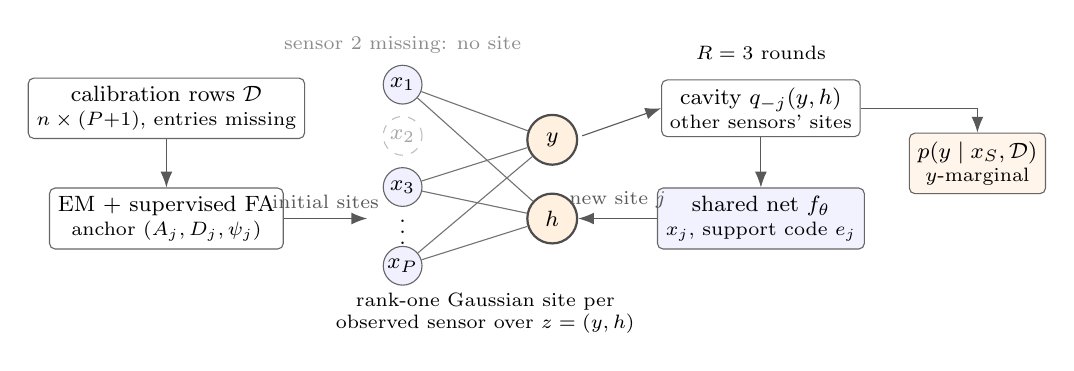
\begin{tikzpicture}[
  font=\footnotesize,
  box/.style={draw=black!60, rounded corners=2pt, align=center, inner sep=3pt, fill=white},
  sens/.style={circle, draw=black!60, minimum size=14pt, inner sep=0pt, fill=blue!6},
  miss/.style={circle, draw=black!25, dashed, minimum size=14pt, inner sep=0pt, text=black!35},
  lat/.style={circle, draw=black!70, thick, minimum size=18pt, inner sep=0pt, fill=orange!12},
  arr/.style={-{Latex[length=2mm]}, black!65},
]
% support and anchor
\node[box, minimum width=2.3cm] (sup) at (0,1.15) {calibration rows $\mathcal{D}$\\[-1pt]{\scriptsize $n\times(P{+}1)$, entries missing}};
\node[box, minimum width=2.3cm] (anc) at (0,-0.25) {EM + supervised FA\\[-1pt]{\scriptsize anchor $(A_j,D_j,\psi_j)$}};
\draw[arr] (sup) -- (anc);
% sensors and latent
\node[sens] (x1) at (3.0,1.45) {$x_1$};
\node[miss] (x2) at (3.0,0.8) {$x_2$};
\node[sens] (x3) at (3.0,0.15) {$x_3$};
\node at (3.0,-0.32) {$\vdots$};
\node[sens] (xP) at (3.0,-0.85) {$x_P$};
\node[lat] (y) at (4.9,0.75) {$y$};
\node[lat] (h) at (4.9,-0.25) {$h$};
\foreach \s in {x1,x3,xP} { \draw[black!55] (\s) -- (y); \draw[black!55] (\s) -- (h); }
\node[font=\scriptsize, text=black!45] at (3.0,1.95) {sensor $2$ missing: no site};
\draw[arr] (anc.east) -- node[above, font=\scriptsize] {initial sites} (2.55,-0.25);
\node[font=\scriptsize, align=center] at (4.05,-1.45) {rank-one Gaussian site per\\observed sensor over $z=(y,h)$};
% refinement loop
\node[box, minimum width=2.0cm] (cav) at (7.55,1.15) {cavity $q_{-j}(y,h)$\\[-1pt]{\scriptsize other sensors' sites}};
\node[box, minimum width=2.0cm, fill=blue!5] (net) at (7.55,-0.25) {shared net $f_\theta$\\[-1pt]{\scriptsize $x_j$, support code $e_j$}};
\draw[arr] (y.east) ++(0.05,0.05) -- (cav.west);
\draw[arr] (cav) -- (net);
\draw[arr] (net.west) -- node[above, font=\scriptsize] {new site $j$} (h.east);
\node[font=\scriptsize] at (7.55,1.85) {$R=3$ rounds};
% output
\node[box, minimum width=1.6cm, fill=orange!8] (out) at (10.3,0.45) {$p(y\mid x_S,\mathcal{D})$\\[-1pt]{\scriptsize $y$-marginal}};
\draw[arr] (cav.east) -| (out.north);
\end{tikzpicture}
\caption{\label{fig:method}Lifted cavity network. A supervised factor analysis estimated from the incomplete
calibration rows gives every sensor a rank-one Gaussian site over the target $y$ and a shared nuisance $h$. Missing
sensors contribute no site, so any subset and any number of sensors are handled by omission. For $R$ rounds, a shared
network replaces each observed sensor's site using its cavity (the posterior from the other sensors) and an encoding
of that sensor's calibration scatter. The prediction is the $y$-marginal of the product.}
\end{figure}


\paragraph{Lifted sites.}
Let $z=(y,h)\in\R^{1+K}$, where $h$ is a $K$-dimensional nuisance with prior $\N(0,I)$ and $y$ has prior
$\N(\mu_y,v_y)$. Write the prior in natural parameters $(\Lambda_0,\eta_0)$. Each observed sensor contributes a
rank-one Gaussian site, which corresponds to a linear-Gaussian measurement $\tilde x_j=w_j^\top z+e_j$ with
$e_j\sim\N(0,\psi_j)$:
\begin{equation}
  \Lambda_j=\frac{w_jw_j^\top}{\psi_j},\qquad \eta_j=\frac{w_j\,o_j}{\psi_j}.
  \label{eq:site}
\end{equation}
The prediction is the $y$-marginal of
\begin{equation}
  q(z\mid x_S)=\N\!\big(z;\Lambda^{-1}\eta,\Lambda^{-1}\big),\qquad
  \Lambda=\Lambda_0+\textstyle\sum_{j\in S}\Lambda_j,\quad \eta=\eta_0+\textstyle\sum_{j\in S}\eta_j .
  \label{eq:product}
\end{equation}

\begin{proposition}[Exactness]\label{prop:exact}
Suppose $x_j=A_jy+D_j^\top h+c_j+e_j$, with independent $e_j\sim\N(0,\psi_j)$ and the priors above. Set $w_j=(A_j,D_j)$
and $o_j=x_j-c_j$. Then \eqref{eq:product} equals $p(z\mid x_S)$ for every $S\subseteq\{1,\dots,P\}$, and its
$y$-marginal is the Bayes predictive for every missingness pattern.
\end{proposition}

Shared noise of rank $K$ is absorbed by $K$ nuisance dimensions, so the obstruction of
Proposition~\ref{prop:scalar} disappears: the lifted product differences out $h$ automatically. Fewer nuisance
dimensions cannot suffice, so the lifting dimension must match the rank of the shared noise:

\begin{proposition}[Lifting dimension]\label{prop:rank}
Let $x=ay+Du+e$ with $y\sim\N(0,1)$, $u\sim\N(0,I_K)$, $D\in\R^{P\times K}$, independent Gaussian $e$, and every
$a_j\neq0$. Suppose
that after deleting any row, $L=[a,D]$ still contains two disjoint nonsingular $(1+K)\times(1+K)$ submatrices, which
holds for almost every $L$ once $P\geq2K+3$. If a product of mask-independent sites of the form \eqref{eq:site} with
$o_j=x_j-c_j$, over $z=(y,h)$ with $h\in\R^{K'}$ and a Gaussian prior, reproduces $p(y\mid x_S)$ for every $S$ with
$|S|\leq2$, then $K'\geq K$.
\end{proposition}

The proof (Appendix~\ref{app:proofs}) shows that the conditionals on single sensors and pairs identify the covariance
of the sensors, which a product of such sites can only represent as a matrix of rank $1+K'$ plus a diagonal; the
identifiability argument of factor analysis~\citep{anderson1956statistical} excludes this when $K'<K$. Our main
synthetic panels ($K=1$, $P=5$) meet the condition, so for products of static sites one nuisance dimension is
necessary and sufficient.

\paragraph{Closed-form initialization from the support.}
Before any learning, we estimate the factor model from $\D$ alone. EM for a Gaussian with missing
entries~\citep{dempster1977em,little2019statistical} gives the joint mean and covariance of $(x,y)$ from the incomplete
calibration rows. Then $A=\mathrm{Cov}(x,y)/\mathrm{Var}(y)$, and principal-factor iterations on the residual
covariance $\mathrm{Cov}(x)-AA^\top\mathrm{Var}(y)$ give $(D,\psi)$~\citep{rubin1982em,tipping1999ppca}. With sensors standardized by
their support statistics, $o_j=\tilde x_j+A_j\mu_y$. We call the resulting predictor \emph{FA-Gaussian}; it is exact
for every mask under the fitted model.

\paragraph{Learned cavity refinement.}
Real sensors are nonlinear, real noise is not exactly factor-structured, and $n=48$ calibration rows make plug-in
estimates noisy. We therefore refine the sites for $R$ rounds. In each round, every observed sensor $j$ removes its
site from \eqref{eq:product} to form the cavity $q_{-j}(z)=\N(m_{-j},V_{-j})$, the posterior over target and nuisance
given the other sensors. The cavity predicts the reading as $\hat x_j=A_j(m_{-j,y}-\mu_y)+D_j^\top m_{-j,h}$, with
variance $v_j=w_j^\top V_{-j}w_j+\psi_j$. A shared two-layer network $f_\theta$ reads the reading $\tilde x_j$, an
encoding $e_j$ of sensor $j$'s calibration scatter, the anchor $(A_j,D_j,\log\psi_j)$, the cavity
$(m_{-j},\log V_{-j,yy},V_{-j,yh})$, the raw and standardized residuals of $\tilde x_j$ against $\hat x_j$, $\log v_j$
and the fraction of observed sensors. It outputs a correction
$(\delta^{\mathrm{off}}_j,\delta^{\mathrm{slope}}_j,\delta^{D}_j,s_j)$, and the site is replaced by the local
linearization of the sensor's response at the cavity mean $\bar y=m_{-j,y}$:
\begin{equation}
  \begin{aligned}
  w_j&=(A_j+\delta^{\mathrm{slope}}_j,\,D_j+\delta^{D}_j), & o_j&=\tilde x_j-g_j(\bar y)+w_{j,y}\bar y,\\
  g_j(\bar y)&=A_j(\bar y-\mu_y)+\delta^{\mathrm{off}}_j, & \psi_j&\leftarrow\psi_j\,e^{4\tanh(s_j/4)} .
  \end{aligned}
  \label{eq:relin}
\end{equation}
The encoding $e_j\in\R^{16}$ is a DeepSets network~\citep{zaheer2017deepsets} over sensor $j$'s calibration scatter,
so $f_\theta$ can recognize a sensor's nonlinearity from the support. The last layer of $f_\theta$ is initialized at
zero.

If $f_\theta$ were replaced by the statistical linear regression of a \emph{known} response function under the cavity,
these rounds would be EP with posterior linearization~\citep{deisenroth2012ep,garciafernandez2015plf}. The network
amortizes the unknown response from the calibration rows, in the spirit of algorithm
unrolling~\citep{gregor2010lista,monga2021unrolling}.

\begin{proposition}[Structural guarantees]\label{prop:struct}
For any parameters $\theta$:
\begin{enumerate}
  \item[(i)] the prediction does not depend on the readings of missing sensors;
  \item[(ii)] permuting sensors together with their calibration columns leaves the prediction unchanged, and the same
  $\theta$ applies for every $P$;
  \item[(iii)] when the last layer of $f_\theta$ is zero, the network equals the FA-Gaussian closed form of its
  anchor, so the minimal training risk over $\theta$ is at most that closed form's.
\end{enumerate}
\end{proposition}

\paragraph{Training.}
We minimize the predictive NLL over episodes drawn from a pool of 60{,}000 synthetic tasks (128 tasks $\times$ 8
queries per step, 20{,}000 AdamW steps with cosine decay, query masks with at most one missing sensor). We use $K=1$
and $R=3$. The model has about 8{,}000 parameters and trains in 15--20 minutes on one CPU core, \Computetrainratio{} times less than the transformer baseline (Table~\ref{tab:compute}). The same recipe trains
every learned baseline except the transformer, which gets fresh tasks at every step.

%=====================================================================
\section{Related work}
\label{sec:related}
%=====================================================================

\textbf{Products of experts} handle missing modalities by omission~\citep{hinton2002poe,wu2018mvae,ma2021smil}; our
negative result says when experts over the target alone are insufficient. \textbf{Learned message passing}, through
learned EP messages~\citep{heess2013learning,eslami2014just,jitkrittum2015kernel} or unrolled
inference~\citep{gregor2010lista,monga2021unrolling}, amortizes inference inside a fixed model; here the model is
unknown and must be read from a small calibration set, and the cavity is over a lifted latent. \textbf{Supervised
learning with missing values}~\citep{rubin1976inference,little2019statistical,josse2019consistency} studies one task
at a time; NeuMiss~\citep{lemorvan2020neumiss} unrolls the Bayes predictor of a Gaussian model but is trained per
dataset and keyed to feature identities. \textbf{In-context prediction} with neural
processes~\citep{garnelo2018cnp,kim2019anp} and prior-fitted networks such as TabPFN and
TabICL~\citep{muller2022pfn,hollmann2023tabpfn,hollmann2025tabpfnv2,qu2025tabicl} uses generic set or transformer
architectures; we compare against such a transformer trained on our task distribution and test lifted sites as its
output layer. \textbf{Fusion under unknown correlations}: covariance intersection~\citep{julier1997ci} bounds fused
errors, and learned fusion with correlated noise~\citep{wang2025ifnet,dong2025difnet} or learned Kalman
gains~\citep{revach2022kalmannet} train per system with fixed sensor sets.

%=====================================================================
\section{Experiments}
\label{sec:experiments}
%=====================================================================
\subsection{Setup}
\label{sec:exp-setup}

\paragraph{Synthetic tasks.}
Each task draws, for every sensor $j$, a response $x_j=a_jy+b_j+0.4\sin(f_jy)+d_ju+\sigma_j\epsilon_j$ with
$a_j=\pm\,\mathcal{U}[0.6,1.8]$ (random sign), $b_j\sim\N(0,0.4^2)$, $f_j\sim\mathcal{U}[0.5,2.5]$, shared-noise
loading $d_j\sim\N(0,0.7^2)$, $\sigma_j\sim\mathcal{U}[0.15,0.8]$ and $y,u,\epsilon_j\sim\N(0,1)$. The support has
$n=48$ rows with 20\% of sensor entries missing at random, and 48 query rows are scored under every mask with $k$
missing sensors (or 20 seeded masks when there are more). The main panel (F1) has 256 fresh tasks with five sensors.
Six further panels of 128 tasks change one factor at a time: 8 or 16 sensors, nonlinearity 0.8 or 0, and 16 or 96
support rows.

\paragraph{Methods.}
\emph{Support-only closed forms:} FA-Gaussian, EM-Gaussian, NL-FA (cubic responses with a tuned curvature penalty and
exact grid inference, a strong plug-in nonlinear model), evidence-tuned Bayesian linear regression (BLR), ridge, and,
post hoc, a Gaussian process. \emph{Learned in-context models}, all trained on the same task family and masks: our
lifted cavity network (8k parameters, three seeds); a residual MLP that receives the same FA anchor and support
encodings (15k parameters, five sensors only); the scalar-cavity network of \S\ref{sec:scalar}; and a TabPFN-v2-style
cell-token transformer~\citep{hollmann2025tabpfnv2} trained on fresh tasks at every step (203k parameters, 30{,}000
steps). A second transformer was trained on \emph{all} masks, to separate architecture from training coverage.
\emph{Privileged references:} the oracle, and the Bayes-optimal predictive estimated by HMC with the shared nuisance
marginalized analytically (Appendix~\ref{app:baselines}).

\paragraph{Protocol.}
NLL is the primary metric; coverage, CRPS~\citep{gneiting2007scoring} and RMSE are secondary. Intervals are paired
95\% intervals over tasks, with per-task NLL averaged over training seeds. Three evaluation protocols were committed
to version control before their panels existed, and every endpoint is reported (Table~\ref{tab:endpoints},
Appendix~\ref{app:audit}).


\subsection{Synthetic tasks with exact references}
\label{sec:exp-main}

\begin{table}[t]
\centering\small
\caption{\label{tab:main}Main synthetic panel (F1: 256 fresh tasks, five sensors). Mean test NLL by number of missing query sensors; learned models saw at most one missing sensor in training, so $k=2,3$ are unseen patterns. Learned rows average three training seeds (seed s.d.\ $\leq0.002$) except the transformers (one seed). Last column: share of the achievable gap (FA-Gaussian to Bayes-optimal) closed at $k=2$. Best non-privileged entry per column in bold.}
\begin{tabular}{lccccc}
\toprule
Method & $k{=}0$ & $k{=}1$ & $k{=}2$ & $k{=}3$ & Gap closed\\
\midrule
\multicolumn{6}{l}{\emph{Privileged references}}\\
Oracle (true parameters) & $-$0.419 & $-$0.250 & $-$0.026 & 0.287 & --\\
Bayes-optimal (HMC, true prior) & $-$0.334 & $-$0.174 & 0.039 & 0.337 & --\\
\midrule
\multicolumn{6}{l}{\emph{Support-only closed forms}}\\
FA-Gaussian & $-$0.152 & $-$0.011 & 0.177 & 0.439 & 0\%\\
EM-Gaussian & $-$0.048 & 0.037 & 0.195 & 0.441 & $-$13\%\\
NL-FA (cubic, tuned) & $-$0.173 & $-$0.036 & 0.151 & 0.417 & 19\%\\
Bayesian linear regression & 0.111 & 0.091 & 0.214 & 0.450 & $-$26\%\\
Ridge (complete case) & 0.026 & 0.078 & 0.216 & 0.451 & $-$28\%\\
Ridge (mean-imputed) & 0.198 & 0.280 & 0.399 & 0.582 & $-$161\%\\
GP, complete case$^\dagger$ & -- & -- & -- & -- & --\\
\midrule
\multicolumn{6}{l}{\emph{Learned in context (trained on $k\leq1$)}}\\
\textbf{Lifted cavity (ours)}, 8k & \textbf{$-$0.265} & \textbf{$-$0.112} & \textbf{0.097} & \textbf{0.395} & 58\%\\
Transformer (TabPFN-v2 style), 203k & $-$0.246 & $-$0.084 & 0.131 & 0.424 & 34\%\\
Residual MLP on FA anchor, 15k & $-$0.236 & $-$0.087 & 0.114 & 0.397 & 46\%\\
Scalar-cavity network, 3k & 0.055 & 0.178 & 0.336 & 0.555 & $-$115\%\\
\emph{Transformer, trained on all masks} & $-$0.237 & $-$0.076 & 0.132 & 0.411 & 33\%\\
\bottomrule
\end{tabular}
\end{table}


\begin{figure}[t]
\centering
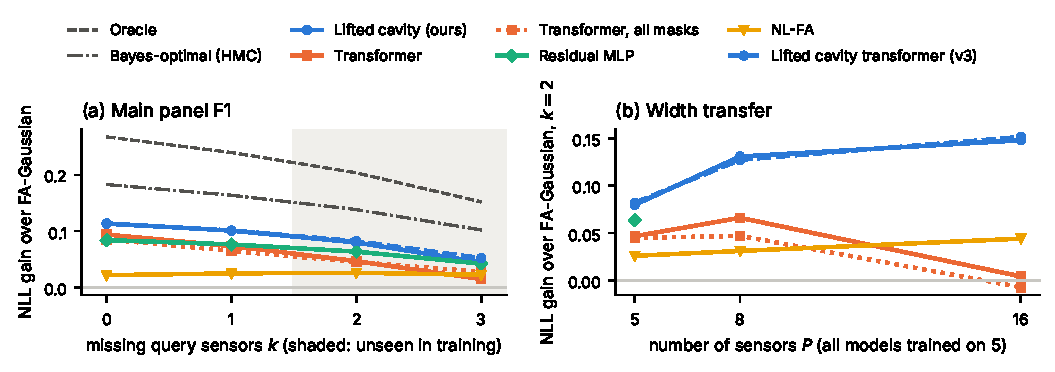
\includegraphics[width=\linewidth]{figures/main.pdf}
\caption{\label{fig:main}NLL gain over the closed-form FA-Gaussian anchor (higher is better). (a) Main panel F1 by
number of missing query sensors; shaded patterns were never seen in training. Grey lines are the privileged oracle and
the sign-conditioned HMC reference. (b) Width transfer with two missing sensors: every learned model was trained on five
sensors, and the residual MLP exists only at $P=5$. Dashed blue: the lifted cavity transformer of
\S\ref{sec:exp-v3}, descriptive on these panels.}
\end{figure}

Table~\ref{tab:main} and Figure~\ref{fig:main}a report the main panel. The lifted cavity network is the best
non-privileged method for every number of missing sensors, including the two- and three-sensor deletions it never saw
in training. With two missing sensors it closes \GapliftOne\% of the reference gap between FA-Gaussian and the
sign-conditioned HMC approximation. Two comparators close less: the residual MLP, which receives the same anchor and support
encodings with twice the parameters (\Gapanchormlp\%), and the tuned nonlinear plug-in model NL-FA (\Gapnlfa\%).
The TabPFN-v2-style transformer has 25 times the parameters and sees fresh tasks at every step. It is still worse
than the lifted cavity network at every number of missing sensors, by \MainkKZeroliftvspfnabs\ to
\MainkKTwoliftvspfnabs\ nats (all intervals exclude zero), and it closes \Gappfn\% of the gap. Training it on every
mask pattern does not change this (\Gappfnall\%): its deficit comes from how efficiently it learns fusion from a
finite training budget, not from unseen patterns. The residual MLP is the closest competitor in this setting. The
lifted cavity network beats it by \MainkKZeroliftvsmlpabs\ nats with all sensors observed and by
\MainkKTwoliftvsmlpabs\ with two missing, and the two tie with three missing.

EM-Gaussian, BLR and both ridges fall below FA-Gaussian; mean imputation is the worst of all.

\subsection{Generalization beyond the training distribution}
\label{sec:exp-shift}

\textbf{Width} (Table~\ref{tab:shift}, Figure~\ref{fig:main}b). The lifted cavity network runs unchanged on 8 and 16 sensors, where it improves on FA-Gaussian by
\SFTwogainfa\ \SFTwogainfaci\ and \SFThreegainfa\ \SFThreegainfaci\ nats with two missing sensors. The residual MLP
cannot run on these panels, and EM-Gaussian degrades as the covariance grows. The transformer also runs at any width, but it gains less over FA-Gaussian as sensors are added. On 16 sensors it is
no better than the closed form, and the lifted cavity network beats it by \SFThreegainpfn\ \SFThreegainpfnci\ nats.

\textbf{Support size.} With 16 calibration rows the transformer degrades sharply, while the lifted cavity network keeps
a \SFSixgainfa\ \SFSixgainfaci\ nat gain over FA-Gaussian; with 96 rows it remains the best method.
\textbf{Stronger nonlinearity} (0.8 instead of 0.4) is the one shift where the transformer competes. It ties the
lifted cavity network with two missing sensors (difference \XFFourkkTwoliftvspfn\ \XFFourkkTwoliftvspfnci) and is
better by \XFFourkkZeroliftvspfnabs\ nats when all sensors are observed: under strong response nonlinearity alone,
Gaussian re-linearization offers no advantage over a generic transformer.
\textbf{Linear sensors.} When the true sensors are linear, FA-Gaussian is nearly the right model and is best; the
learned re-linearization then costs \SFFivegainfaabs\ nats with two missing sensors, and the transformer
\XFFivekkTwopfnvsfaabs.

\subsection{What the lifting buys}
\label{sec:audit}

Ablations on F1 (Table~\ref{tab:ablation}, Appendix~\ref{app:more}) compare components of the small network. \textbf{Lifting} is the
largest factor: scalar sites ($K=0$) with otherwise identical machinery and training lose \AblLiftabs\ \AblLiftci\ nats
with two missing sensors and end up worse than the untrained FA-Gaussian anchor. This supports lifting empirically
under the tested training regime; Proposition~\ref{prop:scalar} does not cover this context-conditioned ablation.
\textbf{Cavity conditioning} adds \AblCavabs\ \AblCavci\ nats on top of lifted static sites. A second
nuisance dimension ($K=2$) changes nothing, as expected for one-factor noise. The scalar-cavity network of the earlier
design, retrained with the same 60{,}000-task recipe, remains far behind FA-Gaussian (Appendix~\ref{app:audit}).

\subsection{Real sensor networks}
\label{sec:exp-real}

\begin{table}[t]
\centering\scriptsize
\setlength{\tabcolsep}{2.5pt}
\caption{\label{tab:real}Real sensor networks: mean test NLL on later, held-out periods. Beijing: 12 target stations $\times$ weekly episodes in 2016--2017 with natural missingness, plus extra dropped sensors. Air Quality: weekly episodes after October 2004, sensor dropout simulated. Fine-tuning uses only earlier periods and one recipe for every model; lifted-cavity and residual-MLP rows average three seeds. Best entry per column in bold. $^\dagger$Post hoc. $^\ddagger$Designed after protocol v2 (Section~\ref{sec:exp-v3}); post hoc here and not bolded.}
\begin{tabular}{lccccccc}
\toprule
Method & \multicolumn{3}{c}{Beijing PM$_{2.5}$ (11 stations)} & \multicolumn{2}{c}{Air Quality CO} & \multicolumn{2}{c}{Air Quality NO$_2$}\\
 & natural & $+3$ & $+6$ & $k{=}0$ & $k{=}2$ & $k{=}0$ & $k{=}2$\\
\midrule
EM-Gaussian & 1.032 & 0.742 & 0.569 & 0.074 & 0.085 & $-$0.237 & $-$0.175\\
FA-Gaussian & 0.677 & 0.615 & 0.562 & 0.052 & 0.116 & $-$0.196 & $-$0.155\\
NL-FA & 0.938 & 0.744 & 0.610 & 0.144 & 0.091 & $-$0.090 & $-$0.142\\
Bayesian linear regression & 0.399 & 0.406 & 0.442 & 1.037 & 0.216 & $-$0.055 & $-$0.178\\
Ridge (complete case) & 0.425 & 0.432 & 0.458 & 0.824 & 0.208 & $-$0.200 & $-$0.176\\
GP, complete case$^\dagger$ & 1.884 & 1.312 & 0.934 & 3.364 & 0.503 & 25.217 & $-$0.198\\
$k$-nearest neighbours$^\dagger$ & 0.508 & 0.514 & 0.540 & 0.571 & 0.353 & $-$0.010 & $-$0.063\\
\midrule
Lifted cavity, zero-shot & 0.826 & 0.661 & 0.561 & 0.044 & 0.129 & $-$0.350 & $-$0.233\\
Transformer, zero-shot & 0.958 & 0.743 & 0.687 & $-$0.017 & 0.081 & $-$0.360 & $-$0.231\\
\midrule
\textbf{Lifted cavity, fine-tuned (ours)} & 0.205 & 0.237 & 0.305 & $-$0.040 & 0.008 & $-$0.412 & $-$0.337\\
\quad no synthetic pretraining & 0.247 & 0.279 & 0.344 & $-$0.001 & $-$0.006 & $-$0.419 & $-$0.316\\
\quad no cavity input & 0.259 & 0.286 & 0.349 & $-$0.086 & $-$0.028 & $-$0.423 & $-$0.332\\
\quad scalar sites ($K=0$) & 0.215 & 0.252 & 0.347 & $-$0.026 & $-$0.003 & $-$0.359 & $-$0.302\\
Transformer, fine-tuned & \textbf{0.087} & \textbf{0.121} & \textbf{0.236} & \textbf{$-$0.163} & \textbf{$-$0.052} & \textbf{$-$0.485} & \textbf{$-$0.381}\\
Residual MLP, fine-tuned & -- & -- & -- & 0.025 & 0.110 & $-$0.246 & $-$0.147\\
\emph{Lifted cavity transformer, fine-tuned}$^\ddagger$ & 0.122 & 0.160 & 0.259 & $-$0.099 & $-$0.027 & $-$0.404 & $-$0.359\\
\bottomrule
\end{tabular}
\end{table}


\paragraph{Beijing multi-site air quality~\citep{zhang2017beijing}.}
The task is to predict log PM$_{2.5}$ at each of 12 monitoring stations from the other 11, using hourly data with
natural missingness. This tests contemporaneous missing-station interpolation, rather than low-cost-device calibration
or future forecasting. Each episode is one station and one week, with 48 labeled support hours and 48 query hours. The
test period (2016-01 to 2017-02, \Rbeijingepisodes\ episodes) was never examined before protocol v2 was committed.
Learned models are fine-tuned on episodes from 2013--2015 with one fixed recipe; the protocol's analysis is
cluster-robust over weeks.

With 11 sensors and 48 rows, the joint-covariance closed forms overfit, and evidence-tuned BLR is the strongest closed
form. The fine-tuned lifted cavity network improves on it by \RbeijingeZerovsblrabs\ \RbeijingeZerovsblrci\ nats under
natural missingness, and by \RbeijingeSixvsblrabs\ \RbeijingeSixvsblrci\ with six further sensors removed.
The fine-tuned transformer is better still. The lifted cavity network's gain over it is \RbeijingeZerovspfn\
\RbeijingeZerovspfnci\ nats under natural missingness and \RbeijingeSixvspfn\ \RbeijingeSixvspfnci\ with six sensors
removed, so endpoint E4b fails. Before fine-tuning the order is reversed: zero-shot, the lifted cavity network is ahead
by \RbeijingeSixzsliftvspfnabs\ \RbeijingeSixzsliftvspfnci\ nats with six sensors removed. Fine-tuning improves the
transformer by more than it improves the lifted network (Table~\ref{tab:real}).

Synthetic pretraining helps: the same network fine-tuned from initialization is \RbeijingeZerovsnopreabs\ nats
worse \RbeijingeZerovsnopreci.

\paragraph{UCI Air Quality~\citep{devito2008airquality}.}
Five metal-oxide sensors on one device predict the reference analyzers' log CO and log NO$_2$, in weekly episodes
after October 2004. These weeks were examined in protocol v1, so this is secondary evidence.
With two simulated missing sensors, the fine-tuned lifted cavity network improves on FA-Gaussian by
\RairqcoeTwovsfa\ \RairqcoeTwovsfaci\ nats for CO and \RairqnoTwoeTwovsfa\ \RairqnoTwoeTwovsfaci\ for NO$_2$. The
fine-tuned transformer is again better: the lifted network's gain over it is \RairqcoeTwovspfn\ \RairqcoeTwovspfnci\
(CO) and \RairqnoTwoeTwovspfn\ \RairqnoTwoeTwovspfnci\ (NO$_2$). On CO, the cavity input stops helping after
fine-tuning.

\paragraph{Why the transformer wins on real data.}
The lifted network underfits rather than overfits: on the Beijing fine-tuning episodes, the transformer's final
training NLL is \FTbeijingtraingap\ nats lower, about the size of the test gap. Post-hoc variants do not close the gap
on Beijing (Table~\ref{tab:explore}; natural missingness, transformer \RbeijingeZerovalftpfn): a second nuisance dimension scores \Xplifttwo\
and five times more fine-tuning steps \Xpliftlong, against \Xpliftone\ for the same seed with the standard recipe.
Nor is the edge that of a flexible per-episode regression: a Gaussian process fitted to each episode's calibration
rows is the worst method on Air Quality (\RairqcoeZerovalgp\ nats for CO with all sensors observed). These point to
the Gaussian site family itself. Gaussian sites with per-sensor re-linearization are a strong prior for synthetic
factor noise, but real stations share structure they cannot express, and a generic model learns it from a few
thousand real episodes: fine-tuning improves the transformer by \FTbeijingpfngain\ nats on Beijing and the lifted
network by \FTbeijingliftgain.


\subsection{Lifted sites as a transformer output layer (protocol v3)}
\label{sec:exp-v3}

Protocol v2 left a split: structure wins on synthetic tasks, the transformer on real networks after fine-tuning. The
\emph{lifted cavity transformer} (LCT; \S\ref{sec:method-lct}) keeps the transformer's backbone, recipe and seed, with
a lifted probabilistic readout. Because the hypothesis was formed after the v2 results, v3 uses new panels (G1,
five sensors; G3, sixteen) and two Beijing pollutants never scored before (NO$_2$ and CO), and its four endpoints were
committed before any of these existed (Table~\ref{tab:endpoints}).

\begin{table}[t]
\centering\scriptsize
\setlength{\tabcolsep}{3pt}
\caption{\label{tab:v3}Protocol v3 (new panels and targets). Mean test NLL. G1: 256 fresh five-sensor tasks by number of missing query sensors $k$; G3: 128 fresh 16-sensor tasks, $k=2$. Beijing: log NO$_2$ and log CO at each station from the other 11 stations, 2016--2017, natural missingness and six further sensors removed; learned models fine-tuned with the recipe of protocol v2 (the all-mask transformer was not fine-tuned). Best entry per column in bold.}
\begin{tabular}{lccccccccc}
\toprule
 & \multicolumn{4}{c}{G1, $P{=}5$} & G3 & \multicolumn{2}{c}{Beijing NO$_2$} & \multicolumn{2}{c}{Beijing CO}\\
Method & $k{=}0$ & $k{=}1$ & $k{=}2$ & $k{=}3$ & $P{=}16$ & natural & $+6$ & natural & $+6$\\
\midrule
FA-Gaussian & \textbf{$-$0.189} & \textbf{$-$0.054} & \textbf{0.129} & \textbf{0.396} & \textbf{$-$0.806} & 0.684 & 0.506 & -- & --\\
Bayesian linear regression & 0.013 & 0.022 & 0.153 & 0.401 & 0.063 & \textbf{0.275} & \textbf{0.365} & -- & --\\
\midrule
Lifted cavity network, 8k & -- & -- & -- & -- & -- & -- & -- & -- & --\\
Transformer, 203k & -- & -- & -- & -- & -- & -- & -- & -- & --\\
Transformer, all masks, 203k & -- & -- & -- & -- & -- & -- & -- & -- & --\\
\textbf{Lifted cavity transformer}, 203k & -- & -- & -- & -- & -- & -- & -- & -- & --\\
\bottomrule
\end{tabular}
\end{table}


\noindent On the fresh synthetic panels, the lifted output layer helps the transformer (Table~\ref{tab:v3}). With two
missing sensors the LCT beats the transformer with the identical backbone, recipe and seed by
\VthreeGOnekTwolctvspfnabs\ \VthreeGOnekTwolctvspfnci\ nats on G1 and \VthreeGThreekTwolctvspfnabs\
\VthreeGThreekTwolctvspfnci\ on sixteen sensors (E5, E6 pass). It matches the small lifted network on five sensors
(\VthreeGOnekTwolctvslift\ \VthreeGOnekTwolctvsliftci) and exceeds it on sixteen (\VthreeGThreekTwolctvslift\
\VthreeGThreekTwolctvsliftci), and it learns faster: its training NLL reaches the transformer's final value after
\Trainlctreach\ of 30{,}000 steps (Figure~\ref{fig:training}). On the v2 panels (descriptive) it closes \Gaplct\% of
the F1 gap (lifted network \GapliftOne\%) but inherits part of the transformer's degradation with 16 calibration rows.
\input{exp_v3_real}



\subsection{Pre-registered endpoints and calibration}
\label{sec:exp-endpoints}

Table~\ref{tab:endpoints} lists every pre-registered endpoint of protocols v2 and v3. Five of six v2 endpoints pass;
the failure, E4b, is the real-data comparison with the fine-tuned transformer. All five v1 endpoints passed
(Appendix~\ref{app:audit}). Three of the four v3 endpoints pass; the failure, E7b, is non-inferiority to the fine-tuned transformer on Beijing
NO$_2$, where the interval is wide.
 Learned models are close to nominal 90\% coverage (lifted
cavity network \CalliftOneFcov\ on F1, \CalliftOneBcov\ on Beijing), while the closed forms under-cover
(Table~\ref{tab:calib}).



%=====================================================================
\section{Limitations}
\label{sec:limits}
%=====================================================================
\textbf{Scope.} The exact and Bayes-optimal references exist only for our generator (one-factor shared noise, a
sinusoidal response nonlinearity, Gaussian targets), and the shift panels vary width, nonlinearity and support size
within it. On the Air Quality device, per-sensor dropout is simulated because its own outages remove all sensors at
once. In Beijing, natural missingness is real but rare (\Rbeijingnatmiss\% of query readings), and larger deletions
are simulated. The gas-sensor-drift benchmark could not separate methods because heavy outliers dominate Gaussian
likelihoods (Appendix~\ref{app:audit}).
\textbf{Model class.} Gaussian sites over a low-dimensional latent cannot represent multimodal posteriors, and on real
networks they underfit (\S\ref{sec:exp-real}). We used $K=1$ throughout.
\textbf{Baselines.} Each transformer was trained once, with a CPU budget (203k parameters, 30{,}000 steps). Pretrained
tabular foundation models (TabPFN~v2, TabICL) could not be run in our sandbox; we provide a script but report no
numbers for them.


%=====================================================================
\section{Conclusion}
%=====================================================================
Products of experts over the target handle missing sensors by construction but provably mishandle shared noise;
Gaussian sites over the target and a nuisance of the noise's rank are necessary and sufficient for factor noise. A
small lifted cavity network learns fusion more efficiently than a 25-times-larger transformer trained on the same
tasks and extrapolates to unseen missingness patterns and wider sensor sets, but on real networks it underfits and a
fine-tuned transformer is better. As the transformer's output layer, lifted sites keep the extrapolation and recover most of that gap on the Beijing
network and about half on the Air Quality device; closing the rest, richer site families and vector targets are
natural next steps.



\bibliographystyle{plainnat}
\bibliography{references}

\clearpage
\appendix
\section{Proofs}
\label{app:proofs}

\paragraph{Proposition~\ref{prop:scalar}.}
Under the model, $p(x_j\mid y)=\N(x_j;a_jy,c_j)$ with $c_j=d_j^2+\sigma_j^2$.

If $q(y\mid x_j)=p(y\mid x_j)$ for all $x_j$, then $p(y)\,t_j(y;x_j)\propto p(y)\,p(x_j\mid y)$ as functions of $y$.
Hence $t_j(y;x_j)=\kappa_j(x_j)\,p(x_j\mid y)$, which is Gaussian in $y$ with precision $a_j^2/c_j>0$. For a pair, $q$
is therefore the naive-Bayes posterior $p(y)\,p(x_j\mid y)\,p(x_k\mid y)$. Its posterior mean is linear in
$(x_j,x_k)$ with coefficients
\[
  (a_j/c_j,\;a_k/c_k)\,/\,\pi_q, \qquad \pi_q=1+a_j^2/c_j+a_k^2/c_k ,
\]
so the coefficient of $x_j$ has the sign of $a_j$.

The Bayes posterior uses $C=\mathrm{Cov}(x_j,x_k\mid y)$, with off-diagonal entry $d_jd_k$. Its mean coefficients are
$(C^{-1}a)^\top/\pi$, with $\pi=1+a^\top C^{-1}a$. Both posteriors are Gaussian, so they coincide for all $(x_j,x_k)$
if and only if $C^{-1}a=\mathrm{diag}(C)^{-1}a$. Equivalently $a=C\,\mathrm{diag}(C)^{-1}a$, whose off-diagonal
components are $d_jd_k\,a_k/c_k=0$ and $d_jd_k\,a_j/c_j=0$. With $a_ja_k\neq0$ this holds if and only if $d_jd_k=0$.

For the sign flip, take $a=(1,1)$, $d=(1,0.5)$ and $\sigma=(0.05,0.05)$. Then the Bayes coefficient of $x_1$ is
$+0.499$ alone and $-0.959$ in the pair. \hfill$\square$

\paragraph{Proposition~\ref{prop:exact}.}
Given $z=(y,h)$, the readings are independent: $x_j\mid z\sim\N(w_j^\top z+c_j,\psi_j)$. Hence
\[
  p(z\mid x_S)\propto p(z)\prod_{j\in S}\N(x_j;w_j^\top z+c_j,\psi_j).
\]
In natural parameters each factor contributes $w_jw_j^\top/\psi_j$ to the precision and $w_j(x_j-c_j)/\psi_j$ to the
shift, which is \eqref{eq:site} with $o_j=x_j-c_j$. The prior is Gaussian, so the product is the Gaussian
\eqref{eq:product}. This holds for every $S$ because the factors of unobserved sensors are absent from both sides.
Marginalizing $h$ gives $p(y\mid x_S)$. \hfill$\square$

\paragraph{Proposition~\ref{prop:rank}.}
\emph{Step 1: the product is a latent-factor model.} By the computation in the proof of Proposition~\ref{prop:exact}
read backwards, a product of sites \eqref{eq:site} with $o_j=x_j-c_j$ is the exact posterior over $z$ of the model
$M_q$: $z\sim\N(\mu_z,\Sigma_z)$ and, independently given $z$, $x_j\sim\N(w_j^\top z+c_j,\psi_j)$. Its $y$-marginal is
$M_q$'s conditional $p_q(y\mid x_S)$, and $M_q$'s sensor covariance is $\Sigma_q=W\Sigma_zW^\top+\mathrm{diag}(\psi)$
with $W\in\R^{P\times(1+K')}$, so $\Sigma_q-\mathrm{diag}(\psi)$ has rank at most $1+K'$.

\emph{Step 2: conditionals on $|S|\leq2$ identify the covariance.} Write $V=\mathrm{Var}(y)$, $c=\mathrm{Cov}(x,y)$
and $\Sigma=\mathrm{Cov}(x)$. The case $S=\emptyset$ gives $V$. For $S=\{j\}$ the conditional has slope
$\beta_j=c_j/\Sigma_{jj}$ and variance $r_j=V-c_j\beta_j$, and $\beta_j\neq0$ because $c_j=a_j\neq0$. Hence
$c_j=(V-r_j)/\beta_j$ and $\Sigma_{jj}=c_j/\beta_j$. For $S=\{j,k\}$ the slope vector $b\neq0$ solves
$\Sigma_{\{jk\}}b=(c_j,c_k)$, and whichever entry of $b$ is non-zero determines $\Sigma_{jk}$ from one row. Since
$M_q$ has the same conditionals, the same formulas apply to it, so $\Sigma_q=\Sigma=LL^\top+\mathrm{diag}(\sigma^2)$.

\emph{Step 3: fewer factors cannot reproduce $\Sigma$.} Let $r=1+K$, so $LL^\top$ has rank $r$. Suppose
$\Sigma=G+\Psi'$ with $\Psi'$ diagonal and $\mathrm{rank}(G)\leq r$. Fix a row $i$ and two disjoint row sets $I_1,I_2$
not containing $i$ with $L_{I_1},L_{I_2}$ nonsingular. In the $(r+1)\times(r+1)$ submatrix of $\Sigma$ with rows
$\{i\}\cup I_1$ and columns $\{i\}\cup I_2$, every entry except $(i,i)$ lies off the diagonal, so it is shared by $G$
and $LL^\top$. Both $G$ and $LL^\top$ have rank at most $r$, so the corresponding minors vanish. Expanding along entry
$(i,i)$, its cofactor is $\det(L_{I_1}L_{I_2}^\top)\neq0$, so $G_{ii}=(LL^\top)_{ii}$. Hence $G=LL^\top$, which has
rank $r$~\citep{anderson1956statistical}. Applying this to $G=W\Sigma_zW^\top$ from Step 1 gives $1+K'\geq r=1+K$.

For almost every $L$ all $r\times r$ submatrices are nonsingular, and $P\geq2r+1=2K+3$ leaves two disjoint sets of $r$
rows after deleting any row. \hfill$\square$

\paragraph{Proposition~\ref{prop:struct}.}
\begin{itemize}
  \item[(i)] Sites of missing sensors are multiplied by the mask before entering \eqref{eq:product}, and the
  network's per-sensor inputs never include another sensor's raw reading, only cavity statistics built from observed
  sites.
  \item[(ii)] Every operation is applied per sensor with shared weights. EM and principal factors are equivariant to
  permutations of the sensor coordinates, and sums over sensors are permutation-invariant. No input encodes a
  sensor's index or the total number of sensors, except the fraction of observed sensors, which is permutation
  invariant.
  \item[(iii)] With a zero last layer, $\delta^{\mathrm{off}}=\delta^{\mathrm{slope}}=\delta^D=s=0$. Then
  $w_j=(A_j,D_j)$, $\psi_j$ is unchanged and $o_j=\tilde x_j-A_j(\bar y-\mu_y)+A_j\bar y=\tilde x_j+A_j\mu_y$. These
  are the initialization sites, so every round reproduces them and the output is the anchor's FA-Gaussian closed form. The zero point lies
  in the parameter set, so the infimum of the training risk is at most FA-Gaussian's. \hfill$\square$
\end{itemize}

\section{Architecture and training details}
\label{app:arch}

\paragraph{Lifted cavity network ($K=1$, $R=3$, 8{,}004 parameters).}
\begin{itemize}
  \item \textbf{Support encoder.} $\phi:\R^3\to\R^{32}\to\R^{32}$ with tanh, applied to each observed calibration
  entry $(\tilde y_i,\tilde x_{ij},\tilde r_{ij})$. The inputs are the standardized target, the centred reading, and
  the anchor residual scaled by $\sqrt{\psi_j}$. The encoder averages over observed rows and then applies
  $\rho:\R^{33}\to\R^{16}$, where the extra input is the observation rate.
  \item \textbf{Site network.} $f_\theta:\R^{28}\to\R^{64}\to\R^{64}\to\R^{4}$ with tanh and a zero-initialized
  last layer.
  \item \textbf{Anchor.} EM uses 8 iterations with a $10^{-4}$ ridge. Principal factors use 40 iterations, with
  uniquenesses floored at $10^{-3}$. Everything is computed in double precision from the support only.
\end{itemize}

\begin{table}[h]
\centering\small
\caption{\label{tab:compute}Compute. Training on one CPU core (core-hours); inference (ms/task) is single-threaded time per task for 480 queries (ten masks $\times$ 48 rows) on F1. Anchors are precomputed in batch and excluded; the closed-form rows include their unbatched NumPy fits.}
\begin{tabular}{lrrrr}
\toprule
Model & Parameters & Training steps & Core-hours & ms/task\\
\midrule
Lifted cavity network & 8{,}004 & 20{,}000 & 0.22 & 7.2\\
Residual MLP on FA anchor & 15{,}490 & 20{,}000 & 0.20 & 1.2\\
Transformer (TabPFN-v2 style) & 202{,}562 & 30{,}000 & 3.11 & 42.9\\
Lifted cavity transformer & 202{,}822 & 30{,}000 & 3.15 & 55.7\\
FA-Gaussian (closed form) & -- & -- & -- & 38.3\\
NL-FA (closed form) & -- & -- & -- & 34.4\\
\bottomrule
\end{tabular}
\end{table}


\paragraph{Training recipe (all synthetic-trained models except the transformer).}
\begin{itemize}
  \item Pool of 60{,}000 tasks (seed 5150).
  \item Minibatches of 128 tasks $\times$ 8 queries.
  \item AdamW with learning rate $1.8\times10^{-3}$, cosine decay to 10\% and weight decay $10^{-4}$.
  \item Gradient clipping at 5 and 20{,}000 steps.
  \item Seeds 1--3.
\end{itemize}
No hyperparameter search was run for any model.

\paragraph{Controls.}
\begin{itemize}
  \item \textbf{Residual MLP on the same anchor} (15{,}490 parameters). It receives the FA-Gaussian prediction, the
  same per-sensor support encodings (concatenated in sensor order), the readings and mask, and a 55-dimensional
  support summary. It outputs a residual correction to the FA-Gaussian mean and log-variance, and is defined only
  for five sensors.
  \item \textbf{Lifted sites without cavity input.} The same sites with the cavity statistics removed.
  \item \textbf{1-D sites} ($K=0$). The same machinery, with sites over $y$ only.
  \item \textbf{Repository cavity network.} The three-round scalar-cavity architecture of
  Appendix~\ref{app:audit}, retrained with the shared recipe.
\end{itemize}

\paragraph{Transformer baseline (202{,}562 parameters).}
The transformer follows TabPFN~v2~\citep{hollmann2025tabpfnv2}:
\begin{itemize}
  \item every cell is a token, embedded by a linear map of its value or by a learned missing-value token;
  \item sensors receive random per-task feature embeddings, so the model is width-agnostic and permutation
  equivariant in distribution;
  \item the target column has its own embedding, and query targets use a learned token;
  \item each of 4 blocks alternates attention across the columns of a row with attention across rows within a
  column (all rows attend to the support rows only), followed by an MLP ($d=64$, 4 heads, hidden width 128,
  pre-LayerNorm);
  \item targets are standardized by the support mean and standard deviation, and the output is a Gaussian mean and
  log-variance.
\end{itemize}
It was trained on fresh tasks at every step (16 tasks $\times$ 16 queries, AdamW with learning rate $10^{-3}$, 1{,}000
warm-up steps, cosine decay, clipping at 1, 30{,}000 steps), with the same query masks as the other models. A second
copy (\emph{all masks}) saw query masks with 0--4 missing sensors, drawn uniformly. Evaluation uses a fixed seed for
the random feature embeddings.

\paragraph{Lifted cavity transformer (protocol v3, 202{,}822 parameters).}
The backbone is the transformer above, unchanged. Its output head is replaced by a zero-initialized linear map from
each query cell's final token to four numbers $(\delta^{\mathrm{off}}_j,\delta^{\mathrm{slope}}_j,\delta^{D}_j,s_j)$,
used exactly as in \eqref{eq:relin} with the linearization point $\bar y$ set to the anchor's closed-form posterior
mean (one round, $K=1$, gradients not propagated through $\bar y$). Readings of missing sensors are replaced by the
missing-value token before the backbone and contribute no site, so they never enter the prediction (a unit test
checks both this and the identity with the anchor's closed form at initialization). Anchors are computed on the fly
for each training task. Training, masks, seed and evaluation are those of the transformer. Figure~\ref{fig:training} compares
the two training curves.

\begin{figure}[h]
\centering
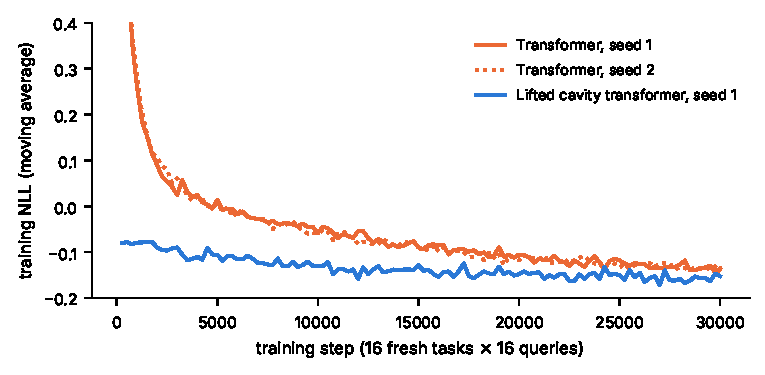
\includegraphics[width=.72\linewidth]{figures/training.pdf}
\caption{\label{fig:training}Training NLL (moving average; fresh tasks with at most one missing sensor) of the
transformer and the lifted cavity transformer, which share backbone, recipe and seed. The lifted output layer starts
at its anchor's closed form, so it begins far lower; the plain transformer must first learn fusion from scratch.}
\end{figure}

\section{Baselines and references}
\label{app:baselines}

\paragraph{Support-only closed forms.}
\begin{itemize}
  \item \textbf{EM-Gaussian:} the conditional of $y$ given $x_S$ under the EM joint Gaussian (40 iterations).
  \item \textbf{FA-Gaussian:} the closed form of \S\ref{sec:method}, with EM run for 40 iterations. The networks'
  anchors use 8 iterations and no variance inflation, so the reported FA-Gaussian is a slightly stronger baseline than
  the untrained networks (on F1 with two missing sensors, \FfaOnekc{} against \Untrainedkc).
  \item \textbf{NL-FA:} per-sensor cubic response curves in the standardized target. The intercept and slope are
  unpenalized; the curvature terms are ridge-penalized ($\lambda=100$) and clamped to the support's target range for
  linear extrapolation. The residual covariance has a one-factor structure. Exact inference is done on a 401-point
  grid. The degree and $\lambda$ were tuned on the development panel only: free degree selection by leave-one-out
  produced catastrophic extrapolation.
  \item \textbf{BLR:} evidence-maximized Bayesian linear regression~\citep{mackay1992bayesian} on complete-case
  rows, with predictive variance including parameter uncertainty.
  \item \textbf{Ridge:} complete-case ridge with leave-one-out residual variance, and the original mean-imputed ridge.
  \item \textbf{Gaussian process (post hoc):} for each episode and observed-sensor set, an ARD squared-exponential
  kernel plus white noise on the complete-case calibration rows, with hyperparameters by type-II maximum likelihood
  (one restart).
  \item \textbf{$k$-nearest neighbours (post hoc):} on the standardized observed sensors of complete-case calibration
  rows, with $k\in\{1,2,3,5,7,10\}$ chosen per episode and sensor set by leave-one-out NLL on the support and the
  leave-one-out mean squared error as predictive variance.
\end{itemize}
EM-Gaussian, FA-Gaussian and ridge inflate their predictive variance by $n/(n-|S|-1)$.

\paragraph{Bayes-optimal ceiling.}
The ceiling is HMC~\citep{neal2011hmc} over the 25 (or $5P$) task parameters. It uses the true priors, transformed to
unconstrained coordinates. The shared nuisance is marginalized analytically through a rank-one-plus-diagonal
covariance, using only the observed entries of each calibration row. The sign of each $a_j$ is fixed by the support
correlation, which is unambiguous because $|a_j|\geq0.6$.

The sampler runs 4 chains per task, each started from a MAP fit. Warm-up has two phases: step-size adaptation (target
acceptance $0.75$) and diagonal mass-matrix estimation from 150 iterations, followed by 150 more adaptation
iterations. We keep 50 draws per chain, thinned by 4, with 12 leapfrog steps.

The predictive density of a query uses the samples exactly, including the query's own reweighting:
$p(y\mid x_S,\D)=\sum_m p(y,x_S\mid\theta_m)/\sum_m p(x_S\mid\theta_m)$, with $p(x_S\mid\theta_m)$ by trapezoid
quadrature on 301 points. On every panel where it was run, R-hat on identifiable parameters was below 1.1 for at
least 99.9\% of parameters. Run with the true parameters, the predictive formula reproduces the exact oracle to
within $2\times10^{-3}$ nats (a unit test).

\section{Protocols and audit trail}
\label{app:audit}
\paragraph{How the method arose.}
The lifted cavity network replaced an earlier design that failed. That design was a three-round EP-style network whose
sites live on $y$ alone and are updated from the scalar cavity of $y$. It was evaluated under pre-registered gates on
the same synthetic family. Its first version collapsed to the prior during training. A repaired version, with sites
initialized from support moments, trained successfully but was beaten by a ridge regression. On that panel the
oracle, the ridge control and the best repaired seed scored:

\begin{center}\small
\begin{tabular}{lr}
\toprule
Method & NLL, two sensors missing\\
\midrule
Oracle & $-0.046$\\
Ridge control & $0.396$\\
Repaired scalar-cavity network (best seed) & $0.403$\\
\bottomrule
\end{tabular}
\end{center}

Computing the oracle exposed three problems. First, the control was weak: it mean-imputed missing calibration
entries, and a support-only EM or factor-analysis Gaussian scores 0.168 or 0.156. Second, scalar sites are
structurally limited (\S\ref{sec:scalar}). Third, the learners were starved: 512 reused tasks and 3{,}000 updates.
Retraining the scalar-cavity architecture with our recipe (60{,}000 tasks, 20{,}000 steps) improves it by only about
0.05 nats, and on F1 it remains \Ablrepocavityfreshvsfaabs\ nats worse than the untrained FA-Gaussian (\S\ref{sec:audit}).

\paragraph{Protocol v1.}
After development on panels that are now retired, five endpoints were committed to version control before their
panels were generated:
\begin{itemize}
  \item fresh synthetic tasks, against FA-Gaussian and against the residual MLP;
  \item 8-sensor transfer;
  \item stronger nonlinearity;
  \item a new real target (NO$_2$ on the Air Quality device).
\end{itemize}
All five passed (Table~\ref{tab:v1}). Each endpoint was evaluated once, and no model was retrained after the commit.

\begin{table}[h]
\centering\small
\caption{\label{tab:v1}Protocol v1 endpoints (two missing sensors; positive gain favours the lifted cavity network; pass requires gain $\geq0.01$ and a positive lower bound).}
\begin{tabular}{llcc}
\toprule
Endpoint & Comparison & Gain [95\% CI] & Result\\
\midrule
E1 & Fresh tasks, vs FA-Gaussian & $+$0.074 [$+$0.064, $+$0.084] & pass\\
E2 & Fresh tasks, vs residual MLP & $+$0.016 [$+$0.012, $+$0.020] & pass\\
E3 & 8 sensors, vs FA-Gaussian & $+$0.115 [$+$0.097, $+$0.132] & pass\\
E4 & Nonlinearity 0.8, vs residual MLP & $+$0.028 [$+$0.020, $+$0.036] & pass\\
R1 & Air Quality NO$_2$, 23 later weeks, vs EM-Gaussian & $+$0.112 [$+$0.050, $+$0.173] & pass\\
\bottomrule
\end{tabular}
\end{table}


\paragraph{Protocol v2.}
Protocol v2 was likewise committed before any of its panels or test splits existed. It adds:
\begin{itemize}
  \item the transformer baseline, NL-FA, BLR and the sign-conditioned HMC reference;
  \item wider panels (8 and 16 sensors), and shifts in nonlinearity and support size;
  \item the Beijing benchmark, whose test period had never been scored.
\end{itemize}
NL-FA's settings and BLR's choice as the strongest real-data closed form were fixed on development data
(Appendix~\ref{app:baselines}). The gas-sensor-drift dataset~\citep{vergara2012drift} was examined during development
and then excluded, before any test split was built. Its heavy-tailed sensor outliers made the mean NLL of every
Gaussian method dominated by a few episodes, with mean and median differing by more than 100 nats, so it cannot
separate methods. One deviation was recorded before any Beijing score existed: some query hours have no other station
observed, and complete-case BLR cannot fit zero features, so for an empty sensor set it returns the support mean with
variance $s^2(1+1/n)$, like the other closed forms' prior predictive.

\paragraph{Protocol v3.}
After protocol v2's real-data endpoint failed, protocol v3 was committed before any of its panels or targets existed.
It fixes one model (the lifted cavity transformer of \S\ref{sec:exp-v3}, trained once with the transformer's recipe
and seed and evaluated at its final checkpoint), two new synthetic panels (G1, G3), two Beijing pollutants never
scored by any model (NO$_2$, primary; CO, descriptive), the fine-tuning recipe of protocol v2, and four endpoints
(Table~\ref{tab:endpoints}). The lifted cavity transformer's scores on the v2 panels are descriptive only
(Appendix~\ref{app:more}). Two container restarts interrupted its training before any v3 score existed; it was retrained
from scratch with the same seed, and later runs checkpoint every random state so that a resumed run is bitwise
identical to an uninterrupted one (a unit test). The protocol document logs both events.

\paragraph{Post-hoc analyses.} Everything not named in a protocol is post hoc and labeled as such: the per-episode
Gaussian process and $k$-nearest neighbours, the second training seeds of both transformers, the fine-tuning diagnostics of \S\ref{sec:exp-real}, and the exploratory runs of
Appendix~\ref{app:more}.


\section{Broader impact}
\label{app:impact}
Calibrating low-cost environmental sensors widens access to air-quality monitoring. Overconfident predictions could
mislead exposure decisions, which is why we report coverage alongside likelihood. We recommend validating calibration
on each new deployment before relying on predicted intervals.

\section{Additional results}
\label{app:more}
\begin{table}[t]
\centering\small
\caption{\label{tab:ablation}Ablations on F1 (mean test NLL). Same training recipe for every learned row.}
\begin{tabular}{lcccc}
\toprule
Variant & $k{=}0$ & $k{=}1$ & $k{=}2$ & $k{=}3$\\
\midrule
Lifted cavity, $K=1$ (ours) & $-$0.265 & $-$0.112 & 0.097 & 0.395\\
Lifted cavity, $K=2$ & $-$0.267 & $-$0.112 & 0.098 & 0.397\\
Lifted sites, no cavity input & $-$0.221 & $-$0.074 & 0.123 & 0.399\\
Scalar sites ($K=0$), same machinery & $-$0.070 & 0.061 & 0.232 & 0.473\\
Scalar-cavity network (retrained) & 0.055 & 0.178 & 0.336 & 0.555\\
FA-Gaussian (untrained) & $-$0.152 & $-$0.011 & 0.177 & 0.439\\
\bottomrule
\end{tabular}
\end{table}

\begin{table}[t]
\centering\small
\caption{\label{tab:calib}Calibration and point accuracy. Coverage of the central 90\% predictive interval (target 0.90), continuous ranked probability score (CRPS, lower is better) and RMSE. F1 with two missing sensors; Beijing test with natural missingness (fine-tuned learned models).}
\begin{tabular}{lcccccc}
\toprule
 & \multicolumn{3}{c}{F1, $k=2$} & \multicolumn{3}{c}{Beijing, natural}\\
Method & Cov.\ 90 & CRPS & RMSE & Cov.\ 90 & CRPS & RMSE\\
\midrule
FA-Gaussian & 0.873 & 0.168 & 0.316 & 0.824 & 0.189 & 0.379\\
EM-Gaussian & 0.860 & 0.170 & 0.318 & 0.807 & 0.207 & 0.423\\
BLR & 0.866 & 0.174 & 0.327 & 0.861 & 0.182 & 0.374\\
Lifted cavity (ours) & 0.901 & 0.160 & 0.305 & 0.914 & 0.171 & 0.357\\
Transformer & 0.902 & 0.165 & 0.314 & 0.914 & 0.158 & 0.341\\
Residual MLP & 0.902 & 0.162 & 0.309 & -- & -- & --\\
\bottomrule
\end{tabular}
\end{table}

\begin{table}[h]
\centering\small
\caption{\label{tab:explore}Post-hoc fine-tuning variants on Beijing PM$_{2.5}$ (test period of protocol v2; mean test NLL). Neither more nuisance dimensions nor longer fine-tuning closes the gap to the fine-tuned transformer.}
\begin{tabular}{lccc}
\toprule
Fine-tuned model & natural & $+3$ & $+6$\\
\midrule
Lifted cavity network, standard recipe (seed 1) & 0.207 & 0.237 & 0.304\\
\quad with $K=2$ & 0.205 & 0.239 & 0.300\\
\quad with $5\times$ fine-tuning steps & 0.169 & 0.201 & 0.276\\
Transformer, standard recipe & 0.087 & 0.121 & 0.236\\
\bottomrule
\end{tabular}
\end{table}

\begin{table}[h]
\centering\small
\caption{\label{tab:moreF2}Panel F2 (8 sensors; 128 tasks): mean test NLL by number of missing sensors.}
\begin{tabular}{lcccc}
\toprule
Method & $k{=}0$ & $k{=}1$ & $k{=}2$ & $k{=}3$\\
\midrule
Oracle & $-$0.807 & $-$0.712 & $-$0.598 & $-$0.459\\
FA-Gaussian & $-$0.462 & $-$0.387 & $-$0.296 & $-$0.183\\
EM-Gaussian & 0.032 & $-$0.133 & $-$0.160 & $-$0.120\\
NL-FA & $-$0.485 & $-$0.414 & $-$0.327 & $-$0.215\\
BLR & 0.187 & 0.398 & 0.615 & 0.028\\
Ridge (complete case) & 0.064 & $-$0.003 & $-$0.033 & $-$0.015\\
Lifted cavity (ours) & $-$0.615 & $-$0.530 & $-$0.427 & $-$0.302\\
Lifted cavity, $K=2$ & $-$0.618 & $-$0.531 & $-$0.427 & $-$0.302\\
Lifted sites, no cavity & $-$0.551 & $-$0.469 & $-$0.369 & $-$0.250\\
Scalar sites ($K=0$) & $-$0.295 & $-$0.228 & $-$0.148 & $-$0.057\\
Transformer & $-$0.568 & $-$0.474 & $-$0.362 & $-$0.229\\
Transformer, all masks & $-$0.545 & $-$0.452 & $-$0.343 & $-$0.212\\
Lifted cavity transformer (v3) & $-$0.611 & $-$0.526 & $-$0.423 & $-$0.299\\
\bottomrule
\end{tabular}
\end{table}

\begin{table}[h]
\centering\small
\caption{\label{tab:moreF3}Panel F3 (16 sensors; 128 tasks): mean test NLL by number of missing sensors.}
\begin{tabular}{lcccc}
\toprule
Method & $k{=}0$ & $k{=}1$ & $k{=}2$ & $k{=}3$\\
\midrule
Oracle & $-$1.223 & $-$1.184 & $-$1.142 & $-$1.096\\
FA-Gaussian & $-$0.864 & $-$0.832 & $-$0.797 & $-$0.758\\
EM-Gaussian & 6.300 & 4.851 & 2.977 & 1.553\\
NL-FA & $-$0.910 & $-$0.876 & $-$0.841 & $-$0.803\\
BLR & 0.095 & 0.078 & 0.058 & 0.054\\
Ridge (complete case) & 0.093 & 0.089 & 0.081 & 0.086\\
Lifted cavity (ours) & $-$1.018 & $-$0.982 & $-$0.945 & $-$0.902\\
Lifted cavity, $K=2$ & $-$1.017 & $-$0.981 & $-$0.944 & $-$0.901\\
Lifted sites, no cavity & $-$0.952 & $-$0.916 & $-$0.880 & $-$0.836\\
Scalar sites ($K=0$) & $-$0.658 & $-$0.627 & $-$0.591 & $-$0.554\\
Transformer & $-$0.886 & $-$0.846 & $-$0.801 & $-$0.747\\
Transformer, all masks & $-$0.869 & $-$0.832 & $-$0.790 & $-$0.738\\
Lifted cavity transformer (v3) & $-$1.020 & $-$0.985 & $-$0.949 & $-$0.905\\
\bottomrule
\end{tabular}
\end{table}

\begin{table}[h]
\centering\small
\caption{\label{tab:moreF4}Panel F4 (nonlinearity 0.8; 128 tasks): mean test NLL by number of missing sensors.}
\begin{tabular}{lcccc}
\toprule
Method & $k{=}0$ & $k{=}1$ & $k{=}2$ & $k{=}3$\\
\midrule
Oracle & $-$0.513 & $-$0.331 & $-$0.086 & 0.261\\
FA-Gaussian & 0.050 & 0.170 & 0.334 & 0.568\\
EM-Gaussian & 0.050 & 0.145 & 0.311 & 0.559\\
NL-FA & $-$0.032 & 0.089 & 0.258 & 0.507\\
BLR & 0.208 & 0.188 & 0.331 & 0.568\\
Ridge (complete case) & 0.138 & 0.208 & 0.338 & 0.571\\
Lifted cavity (ours) & $-$0.185 & $-$0.026 & 0.191 & 0.498\\
Lifted cavity, $K=2$ & $-$0.200 & $-$0.035 & 0.186 & 0.497\\
Lifted sites, no cavity & $-$0.068 & 0.075 & 0.261 & 0.519\\
Scalar sites ($K=0$) & $-$0.013 & 0.130 & 0.314 & 0.570\\
Transformer & $-$0.226 & $-$0.043 & 0.191 & 0.503\\
Transformer, all masks & $-$0.221 & $-$0.038 & 0.190 & 0.486\\
Residual MLP & $-$0.107 & 0.039 & 0.235 & 0.508\\
Scalar-cavity network & 0.133 & 0.256 & 0.416 & 0.635\\
Lifted cavity transformer (v3) & $-$0.196 & $-$0.037 & 0.179 & 0.482\\
\bottomrule
\end{tabular}
\end{table}

\begin{table}[h]
\centering\small
\caption{\label{tab:moreF5}Panel F5 (linear sensors; 128 tasks): mean test NLL by number of missing sensors.}
\begin{tabular}{lcccc}
\toprule
Method & $k{=}0$ & $k{=}1$ & $k{=}2$ & $k{=}3$\\
\midrule
Oracle & $-$0.455 & $-$0.288 & $-$0.066 & 0.244\\
FA-Gaussian & $-$0.362 & $-$0.203 & 0.009 & 0.305\\
EM-Gaussian & $-$0.244 & $-$0.142 & 0.034 & 0.308\\
NL-FA & $-$0.337 & $-$0.178 & 0.030 & 0.318\\
BLR & $-$0.135 & $-$0.085 & 0.061 & 0.322\\
Ridge (complete case) & $-$0.169 & $-$0.092 & 0.062 & 0.323\\
Lifted cavity (ours) & $-$0.323 & $-$0.172 & 0.031 & 0.318\\
Lifted cavity, $K=2$ & $-$0.320 & $-$0.170 & 0.033 & 0.318\\
Lifted sites, no cavity & $-$0.343 & $-$0.189 & 0.018 & 0.309\\
Scalar sites ($K=0$) & $-$0.085 & 0.031 & 0.186 & 0.415\\
Transformer & $-$0.278 & $-$0.122 & 0.085 & 0.371\\
Transformer, all masks & $-$0.281 & $-$0.123 & 0.080 & 0.353\\
Residual MLP & $-$0.304 & $-$0.161 & 0.036 & 0.319\\
Scalar-cavity network & 0.052 & 0.161 & 0.302 & 0.505\\
Lifted cavity transformer (v3) & $-$0.319 & $-$0.171 & 0.029 & 0.315\\
\bottomrule
\end{tabular}
\end{table}

\begin{table}[h]
\centering\small
\caption{\label{tab:moreF6}Panel F6 (16 support rows; 128 tasks): mean test NLL by number of missing sensors.}
\begin{tabular}{lcccc}
\toprule
Method & $k{=}0$ & $k{=}1$ & $k{=}2$ & $k{=}3$\\
\midrule
Oracle & $-$0.446 & $-$0.280 & $-$0.060 & 0.252\\
FA-Gaussian & 0.256 & 0.371 & 0.510 & 0.686\\
EM-Gaussian & 24.900 & 4.682 & 1.140 & 0.739\\
NL-FA & 0.314 & 0.388 & 0.496 & 0.661\\
BLR & 0.898 & 0.857 & 3.690 & 0.887\\
Ridge (complete case) & 0.317 & 0.391 & 0.500 & 0.624\\
Lifted cavity (ours) & 0.073 & 0.195 & 0.363 & 0.604\\
Lifted cavity, $K=2$ & 0.156 & 0.250 & 0.392 & 0.614\\
Lifted sites, no cavity & 0.117 & 0.234 & 0.389 & 0.604\\
Scalar sites ($K=0$) & 0.204 & 0.293 & 0.428 & 0.644\\
Transformer & 0.253 & 0.371 & 0.523 & 0.731\\
Transformer, all masks & 0.256 & 0.359 & 0.483 & 0.653\\
Residual MLP & 0.094 & 0.211 & 0.371 & 0.594\\
Scalar-cavity network & 0.345 & 0.439 & 0.565 & 0.750\\
Lifted cavity transformer (v3) & 0.237 & 0.333 & 0.457 & 0.643\\
\bottomrule
\end{tabular}
\end{table}

\begin{table}[h]
\centering\small
\caption{\label{tab:moreF7}Panel F7 (96 support rows; 128 tasks): mean test NLL by number of missing sensors.}
\begin{tabular}{lcccc}
\toprule
Method & $k{=}0$ & $k{=}1$ & $k{=}2$ & $k{=}3$\\
\midrule
Oracle & $-$0.429 & $-$0.264 & $-$0.043 & 0.269\\
FA-Gaussian & $-$0.232 & $-$0.082 & 0.114 & 0.385\\
EM-Gaussian & $-$0.237 & $-$0.086 & 0.112 & 0.385\\
NL-FA & $-$0.276 & $-$0.127 & 0.073 & 0.353\\
BLR & $-$0.178 & $-$0.056 & 0.125 & 0.390\\
Ridge (complete case) & $-$0.163 & $-$0.047 & 0.129 & 0.391\\
Lifted cavity (ours) & $-$0.324 & $-$0.163 & 0.052 & 0.353\\
Lifted cavity, $K=2$ & $-$0.320 & $-$0.159 & 0.056 & 0.357\\
Lifted sites, no cavity & $-$0.275 & $-$0.123 & 0.078 & 0.359\\
Scalar sites ($K=0$) & $-$0.097 & 0.034 & 0.205 & 0.443\\
Transformer & $-$0.295 & $-$0.133 & 0.081 & 0.379\\
Transformer, all masks & $-$0.297 & $-$0.134 & 0.080 & 0.367\\
Residual MLP & $-$0.287 & $-$0.131 & 0.074 & 0.360\\
Scalar-cavity network & 0.047 & 0.161 & 0.309 & 0.516\\
Lifted cavity transformer (v3) & $-$0.329 & $-$0.167 & 0.047 & 0.346\\
\bottomrule
\end{tabular}
\end{table}

\begin{table}[h]
\centering\small
\caption{\label{tab:moreairqco}Air Quality CO: mean test NLL for every number of simulated missing sensors (23 later weeks).}
\begin{tabular}{lcccc}
\toprule
Method & $k{=}0$ & $k{=}1$ & $k{=}2$ & $k{=}3$\\
\midrule
EM-Gaussian & 0.074 & 0.063 & 0.085 & 0.146\\
FA-Gaussian & 0.052 & 0.086 & 0.116 & 0.154\\
NL-FA & 0.144 & 0.120 & 0.091 & 0.124\\
Bayesian linear regression & 1.037 & 0.433 & 0.216 & 0.202\\
Ridge (complete case) & 0.824 & 0.337 & 0.208 & 0.210\\
GP, complete case$^\dagger$ & 3.364 & 1.056 & 0.503 & 0.146\\
$k$-nearest neighbours$^\dagger$ & 0.571 & 0.391 & 0.353 & 0.274\\
Lifted cavity, zero-shot & 0.044 & 0.064 & 0.129 & 0.160\\
Transformer, zero-shot & $-$0.017 & $-$0.006 & 0.081 & 0.154\\
\textbf{Lifted cavity, fine-tuned (ours)} & $-$0.040 & $-$0.031 & 0.008 & 0.077\\
\quad no synthetic pretraining & $-$0.001 & $-$0.014 & $-$0.006 & 0.077\\
\quad no cavity input & $-$0.086 & $-$0.065 & $-$0.028 & 0.038\\
\quad scalar sites ($K=0$) & $-$0.026 & $-$0.021 & $-$0.003 & 0.075\\
Transformer, fine-tuned & $-$0.163 & $-$0.149 & $-$0.052 & 0.036\\
Residual MLP, fine-tuned & 0.025 & 0.061 & 0.110 & 0.160\\
\bottomrule
\end{tabular}
\end{table}

\begin{table}[h]
\centering\small
\caption{\label{tab:moreairqno2}Air Quality NO$_2$: mean test NLL for every number of simulated missing sensors (23 later weeks).}
\begin{tabular}{lcccc}
\toprule
Method & $k{=}0$ & $k{=}1$ & $k{=}2$ & $k{=}3$\\
\midrule
EM-Gaussian & $-$0.237 & $-$0.174 & $-$0.175 & $-$0.168\\
FA-Gaussian & $-$0.196 & $-$0.173 & $-$0.155 & $-$0.162\\
NL-FA & $-$0.090 & $-$0.102 & $-$0.142 & $-$0.169\\
Bayesian linear regression & $-$0.055 & $-$0.214 & $-$0.178 & $-$0.160\\
Ridge (complete case) & $-$0.200 & $-$0.230 & $-$0.176 & $-$0.145\\
GP, complete case$^\dagger$ & 25.217 & 0.696 & $-$0.198 & $-$0.258\\
$k$-nearest neighbours$^\dagger$ & $-$0.010 & $-$0.020 & $-$0.063 & $-$0.128\\
Lifted cavity, zero-shot & $-$0.350 & $-$0.295 & $-$0.233 & $-$0.176\\
Transformer, zero-shot & $-$0.360 & $-$0.310 & $-$0.231 & $-$0.136\\
\textbf{Lifted cavity, fine-tuned (ours)} & $-$0.412 & $-$0.366 & $-$0.337 & $-$0.273\\
\quad no synthetic pretraining & $-$0.419 & $-$0.365 & $-$0.316 & $-$0.248\\
\quad no cavity input & $-$0.423 & $-$0.375 & $-$0.332 & $-$0.275\\
\quad scalar sites ($K=0$) & $-$0.359 & $-$0.337 & $-$0.302 & $-$0.231\\
Transformer, fine-tuned & $-$0.485 & $-$0.429 & $-$0.381 & $-$0.294\\
Residual MLP, fine-tuned & $-$0.246 & $-$0.198 & $-$0.147 & $-$0.106\\
\bottomrule
\end{tabular}
\end{table}



\clearpage
\section*{NeurIPS Paper Checklist}




\begin{enumerate}

\item {\bf Claims}
    \item[] Question: Do the main claims made in the abstract and introduction accurately reflect the paper's contributions and scope?
    \item[] Answer: \answerYes{}
    \item[] Justification: The abstract and introduction state the scope: synthetic tasks from one generator family with exact oracle and sign-conditioned HMC references, and two real sensor networks; limitations are in Section~\ref{sec:limits}.
    \item[] Guidelines:
    \begin{itemize}
        \item The answer \answerNA{} means that the abstract and introduction do not include the claims made in the paper.
        \item The abstract and/or introduction should clearly state the claims made, including the contributions made in the paper and important assumptions and limitations. A \answerNo{} or \answerNA{} answer to this question will not be perceived well by the reviewers. 
        \item The claims made should match theoretical and experimental results, and reflect how much the results can be expected to generalize to other settings. 
        \item It is fine to include aspirational goals as motivation as long as it is clear that these goals are not attained by the paper. 
    \end{itemize}

\item {\bf Limitations}
    \item[] Question: Does the paper discuss the limitations of the work performed by the authors?
    \item[] Answer: \answerYes{}
    \item[] Justification: Section~\ref{sec:limits} discusses the synthetic family, the real-data scope, Gaussian sites, the transformer compute budget and the untested pretrained tabular foundation models.
    \item[] Guidelines:
    \begin{itemize}
        \item The answer \answerNA{} means that the paper has no limitation while the answer \answerNo{} means that the paper has limitations, but those are not discussed in the paper. 
        \item The authors are encouraged to create a separate ``Limitations'' section in their paper.
        \item The paper should point out any strong assumptions and how robust the results are to violations of these assumptions (e.g., independence assumptions, noiseless settings, model well-specification, asymptotic approximations only holding locally). The authors should reflect on how these assumptions might be violated in practice and what the implications would be.
        \item The authors should reflect on the scope of the claims made, e.g., if the approach was only tested on a few datasets or with a few runs. In general, empirical results often depend on implicit assumptions, which should be articulated.
        \item The authors should reflect on the factors that influence the performance of the approach. For example, a facial recognition algorithm may perform poorly when image resolution is low or images are taken in low lighting. Or a speech-to-text system might not be used reliably to provide closed captions for online lectures because it fails to handle technical jargon.
        \item The authors should discuss the computational efficiency of the proposed algorithms and how they scale with dataset size.
        \item If applicable, the authors should discuss possible limitations of their approach to address problems of privacy and fairness.
        \item While the authors might fear that complete honesty about limitations might be used by reviewers as grounds for rejection, a worse outcome might be that reviewers discover limitations that aren't acknowledged in the paper. The authors should use their best judgment and recognize that individual actions in favor of transparency play an important role in developing norms that preserve the integrity of the community. Reviewers will be specifically instructed to not penalize honesty concerning limitations.
    \end{itemize}

\item {\bf Theory assumptions and proofs}
    \item[] Question: For each theoretical result, does the paper provide the full set of assumptions and a complete (and correct) proof?
    \item[] Answer: \answerYes{}
    \item[] Justification: Assumptions are stated in Propositions~\ref{prop:scalar}--\ref{prop:struct}; complete proofs are in Appendix~\ref{app:proofs}.
    \item[] Guidelines:
    \begin{itemize}
        \item The answer \answerNA{} means that the paper does not include theoretical results. 
        \item All the theorems, formulas, and proofs in the paper should be numbered and cross-referenced.
        \item All assumptions should be clearly stated or referenced in the statement of any theorems.
        \item The proofs can either appear in the main paper or the supplemental material, but if they appear in the supplemental material, the authors are encouraged to provide a short proof sketch to provide intuition. 
        \item Inversely, any informal proof provided in the core of the paper should be complemented by formal proofs provided in appendix or supplemental material.
        \item Theorems and Lemmas that the proof relies upon should be properly referenced. 
    \end{itemize}

    \item {\bf Experimental result reproducibility}
    \item[] Question: Does the paper fully disclose all the information needed to reproduce the main experimental results of the paper to the extent that it affects the main claims and/or conclusions of the paper (regardless of whether the code and data are provided or not)?
    \item[] Answer: \answerYes{}
    \item[] Justification: Appendices~\ref{app:arch} and~\ref{app:baselines} give architectures, recipes and baselines; seeds, panels and endpoints are fixed by three committed protocols (Appendix~\ref{app:audit}).
    \item[] Guidelines:
    \begin{itemize}
        \item The answer \answerNA{} means that the paper does not include experiments.
        \item If the paper includes experiments, a \answerNo{} answer to this question will not be perceived well by the reviewers: Making the paper reproducible is important, regardless of whether the code and data are provided or not.
        \item If the contribution is a dataset and\slash or model, the authors should describe the steps taken to make their results reproducible or verifiable. 
        \item Depending on the contribution, reproducibility can be accomplished in various ways. For example, if the contribution is a novel architecture, describing the architecture fully might suffice, or if the contribution is a specific model and empirical evaluation, it may be necessary to either make it possible for others to replicate the model with the same dataset, or provide access to the model. In general. releasing code and data is often one good way to accomplish this, but reproducibility can also be provided via detailed instructions for how to replicate the results, access to a hosted model (e.g., in the case of a large language model), releasing of a model checkpoint, or other means that are appropriate to the research performed.
        \item While NeurIPS does not require releasing code, the conference does require all submissions to provide some reasonable avenue for reproducibility, which may depend on the nature of the contribution. For example
        \begin{enumerate}
            \item If the contribution is primarily a new algorithm, the paper should make it clear how to reproduce that algorithm.
            \item If the contribution is primarily a new model architecture, the paper should describe the architecture clearly and fully.
            \item If the contribution is a new model (e.g., a large language model), then there should either be a way to access this model for reproducing the results or a way to reproduce the model (e.g., with an open-source dataset or instructions for how to construct the dataset).
            \item We recognize that reproducibility may be tricky in some cases, in which case authors are welcome to describe the particular way they provide for reproducibility. In the case of closed-source models, it may be that access to the model is limited in some way (e.g., to registered users), but it should be possible for other researchers to have some path to reproducing or verifying the results.
        \end{enumerate}
    \end{itemize}


\item {\bf Open access to data and code}
    \item[] Question: Does the paper provide open access to the data and code, with sufficient instructions to faithfully reproduce the main experimental results, as described in supplemental material?
    \item[] Answer: \answerNo{}
    \item[] Justification: Code, checkpoints, per-task scores and protocols are retained in the research repository, and public UCI data have recorded file hashes. An anonymized, independently tested supplementary archive is still pending.
    \item[] Guidelines:
    \begin{itemize}
        \item The answer \answerNA{} means that paper does not include experiments requiring code.
        \item Please see the NeurIPS code and data submission guidelines (\url{https://neurips.cc/public/guides/CodeSubmissionPolicy}) for more details.
        \item While we encourage the release of code and data, we understand that this might not be possible, so \answerNo{} is an acceptable answer. Papers cannot be rejected simply for not including code, unless this is central to the contribution (e.g., for a new open-source benchmark).
        \item The instructions should contain the exact command and environment needed to run to reproduce the results. See the NeurIPS code and data submission guidelines (\url{https://neurips.cc/public/guides/CodeSubmissionPolicy}) for more details.
        \item The authors should provide instructions on data access and preparation, including how to access the raw data, preprocessed data, intermediate data, and generated data, etc.
        \item The authors should provide scripts to reproduce all experimental results for the new proposed method and baselines. If only a subset of experiments are reproducible, they should state which ones are omitted from the script and why.
        \item At submission time, to preserve anonymity, the authors should release anonymized versions (if applicable).
        \item Providing as much information as possible in supplemental material (appended to the paper) is recommended, but including URLs to data and code is permitted.
    \end{itemize}


\item {\bf Experimental setting/details}
    \item[] Question: Does the paper specify all the training and test details (e.g., data splits, hyperparameters, how they were chosen, type of optimizer) necessary to understand the results?
    \item[] Answer: \answerYes{}
    \item[] Justification: Section~\ref{sec:experiments} and Appendices~\ref{app:arch}--\ref{app:baselines} give data generation, training recipes, fine-tuning recipes and evaluation masks.
    \item[] Guidelines:
    \begin{itemize}
        \item The answer \answerNA{} means that the paper does not include experiments.
        \item The experimental setting should be presented in the core of the paper to a level of detail that is necessary to appreciate the results and make sense of them.
        \item The full details can be provided either with the code, in appendix, or as supplemental material.
    \end{itemize}

\item {\bf Experiment statistical significance}
    \item[] Question: Does the paper report error bars suitably and correctly defined or other appropriate information about the statistical significance of the experiments?
    \item[] Answer: \answerYes{}
    \item[] Justification: All comparisons report paired 95\% intervals over tasks or (for Beijing) cluster-robust intervals over weeks; learned models use three training seeds where stated.
    \item[] Guidelines:
    \begin{itemize}
        \item The answer \answerNA{} means that the paper does not include experiments.
        \item The authors should answer \answerYes{} if the results are accompanied by error bars, confidence intervals, or statistical significance tests, at least for the experiments that support the main claims of the paper.
        \item The factors of variability that the error bars are capturing should be clearly stated (for example, train/test split, initialization, random drawing of some parameter, or overall run with given experimental conditions).
        \item The method for calculating the error bars should be explained (closed form formula, call to a library function, bootstrap, etc.)
        \item The assumptions made should be given (e.g., Normally distributed errors).
        \item It should be clear whether the error bar is the standard deviation or the standard error of the mean.
        \item It is OK to report 1-sigma error bars, but one should state it. The authors should preferably report a 2-sigma error bar than state that they have a 96\% CI, if the hypothesis of Normality of errors is not verified.
        \item For asymmetric distributions, the authors should be careful not to show in tables or figures symmetric error bars that would yield results that are out of range (e.g., negative error rates).
        \item If error bars are reported in tables or plots, the authors should explain in the text how they were calculated and reference the corresponding figures or tables in the text.
    \end{itemize}

\item {\bf Experiments compute resources}
    \item[] Question: For each experiment, does the paper provide sufficient information on the computer resources (type of compute workers, memory, time of execution) needed to reproduce the experiments?
    \item[] Answer: \answerYes{}
    \item[] Justification: The reported v1--v3 efficacy experiments ran on two CPU cores; parameters, training time and inference cost are in Table~\ref{tab:compute} (Appendix~\ref{app:arch}). Separate GPU engineering probes do not establish v4 efficacy; its full comparison is pending.
    \item[] Guidelines:
    \begin{itemize}
        \item The answer \answerNA{} means that the paper does not include experiments.
        \item The paper should indicate the type of compute workers CPU or GPU, internal cluster, or cloud provider, including relevant memory and storage.
        \item The paper should provide the amount of compute required for each of the individual experimental runs as well as estimate the total compute. 
        \item The paper should disclose whether the full research project required more compute than the experiments reported in the paper (e.g., preliminary or failed experiments that didn't make it into the paper). 
    \end{itemize}
    
\item {\bf Code of ethics}
    \item[] Question: Does the research conducted in the paper conform, in every respect, with the NeurIPS Code of Ethics \url{https://neurips.cc/public/EthicsGuidelines}?
    \item[] Answer: \answerYes{}
    \item[] Justification: The work uses public environmental sensor data and synthetic data and conforms to the Code of Ethics.
    \item[] Guidelines:
    \begin{itemize}
        \item The answer \answerNA{} means that the authors have not reviewed the NeurIPS Code of Ethics.
        \item If the authors answer \answerNo, they should explain the special circumstances that require a deviation from the Code of Ethics.
        \item The authors should make sure to preserve anonymity (e.g., if there is a special consideration due to laws or regulations in their jurisdiction).
    \end{itemize}


\item {\bf Broader impacts}
    \item[] Question: Does the paper discuss both potential positive societal impacts and negative societal impacts of the work performed?
    \item[] Answer: \answerYes{}
    \item[] Justification: Appendix~\ref{app:impact} discusses benefits for low-cost environmental monitoring and the risk of overconfident predictions; we report calibration.
    \item[] Guidelines:
    \begin{itemize}
        \item The answer \answerNA{} means that there is no societal impact of the work performed.
        \item If the authors answer \answerNA{} or \answerNo, they should explain why their work has no societal impact or why the paper does not address societal impact.
        \item Examples of negative societal impacts include potential malicious or unintended uses (e.g., disinformation, generating fake profiles, surveillance), fairness considerations (e.g., deployment of technologies that could make decisions that unfairly impact specific groups), privacy considerations, and security considerations.
        \item The conference expects that many papers will be foundational research and not tied to particular applications, let alone deployments. However, if there is a direct path to any negative applications, the authors should point it out. For example, it is legitimate to point out that an improvement in the quality of generative models could be used to generate Deepfakes for disinformation. On the other hand, it is not needed to point out that a generic algorithm for optimizing neural networks could enable people to train models that generate Deepfakes faster.
        \item The authors should consider possible harms that could arise when the technology is being used as intended and functioning correctly, harms that could arise when the technology is being used as intended but gives incorrect results, and harms following from (intentional or unintentional) misuse of the technology.
        \item If there are negative societal impacts, the authors could also discuss possible mitigation strategies (e.g., gated release of models, providing defenses in addition to attacks, mechanisms for monitoring misuse, mechanisms to monitor how a system learns from feedback over time, improving the efficiency and accessibility of ML).
    \end{itemize}
    
\item {\bf Safeguards}
    \item[] Question: Does the paper describe safeguards that have been put in place for responsible release of data or models that have a high risk for misuse (e.g., pre-trained language models, image generators, or scraped datasets)?
    \item[] Answer: \answerNA{}
    \item[] Justification: The released models are small task-specific predictors with no foreseeable high risk of misuse.
    \item[] Guidelines:
    \begin{itemize}
        \item The answer \answerNA{} means that the paper poses no such risks.
        \item Released models that have a high risk for misuse or dual-use should be released with necessary safeguards to allow for controlled use of the model, for example by requiring that users adhere to usage guidelines or restrictions to access the model or implementing safety filters. 
        \item Datasets that have been scraped from the Internet could pose safety risks. The authors should describe how they avoided releasing unsafe images.
        \item We recognize that providing effective safeguards is challenging, and many papers do not require this, but we encourage authors to take this into account and make a best faith effort.
    \end{itemize}

\item {\bf Licenses for existing assets}
    \item[] Question: Are the creators or original owners of assets (e.g., code, data, models), used in the paper, properly credited and are the license and terms of use explicitly mentioned and properly respected?
    \item[] Answer: \answerYes{}
    \item[] Justification: The UCI Air Quality and Beijing Multi-Site datasets are CC BY 4.0 and are cited; the TabPFN-v2-style baseline is our own implementation.
    \item[] Guidelines:
    \begin{itemize}
        \item The answer \answerNA{} means that the paper does not use existing assets.
        \item The authors should cite the original paper that produced the code package or dataset.
        \item The authors should state which version of the asset is used and, if possible, include a URL.
        \item The name of the license (e.g., CC-BY 4.0) should be included for each asset.
        \item For scraped data from a particular source (e.g., website), the copyright and terms of service of that source should be provided.
        \item If assets are released, the license, copyright information, and terms of use in the package should be provided. For popular datasets, \url{paperswithcode.com/datasets} has curated licenses for some datasets. Their licensing guide can help determine the license of a dataset.
        \item For existing datasets that are re-packaged, both the original license and the license of the derived asset (if it has changed) should be provided.
        \item If this information is not available online, the authors are encouraged to reach out to the asset's creators.
    \end{itemize}

\item {\bf New assets}
    \item[] Question: Are new assets introduced in the paper well documented and is the documentation provided alongside the assets?
    \item[] Answer: \answerYes{}
    \item[] Justification: Code and checkpoints are documented in the repository README and the protocols.
    \item[] Guidelines:
    \begin{itemize}
        \item The answer \answerNA{} means that the paper does not release new assets.
        \item Researchers should communicate the details of the dataset\slash code\slash model as part of their submissions via structured templates. This includes details about training, license, limitations, etc. 
        \item The paper should discuss whether and how consent was obtained from people whose asset is used.
        \item At submission time, remember to anonymize your assets (if applicable). You can either create an anonymized URL or include an anonymized zip file.
    \end{itemize}

\item {\bf Crowdsourcing and research with human subjects}
    \item[] Question: For crowdsourcing experiments and research with human subjects, does the paper include the full text of instructions given to participants and screenshots, if applicable, as well as details about compensation (if any)? 
    \item[] Answer: \answerNA{}
    \item[] Justification: No crowdsourcing or human subjects.
    \item[] Guidelines:
    \begin{itemize}
        \item The answer \answerNA{} means that the paper does not involve crowdsourcing nor research with human subjects.
        \item Including this information in the supplemental material is fine, but if the main contribution of the paper involves human subjects, then as much detail as possible should be included in the main paper. 
        \item According to the NeurIPS Code of Ethics, workers involved in data collection, curation, or other labor should be paid at least the minimum wage in the country of the data collector. 
    \end{itemize}

\item {\bf Institutional review board (IRB) approvals or equivalent for research with human subjects}
    \item[] Question: Does the paper describe potential risks incurred by study participants, whether such risks were disclosed to the subjects, and whether Institutional Review Board (IRB) approvals (or an equivalent approval/review based on the requirements of your country or institution) were obtained?
    \item[] Answer: \answerNA{}
    \item[] Justification: No human subjects.
    \item[] Guidelines:
    \begin{itemize}
        \item The answer \answerNA{} means that the paper does not involve crowdsourcing nor research with human subjects.
        \item Depending on the country in which research is conducted, IRB approval (or equivalent) may be required for any human subjects research. If you obtained IRB approval, you should clearly state this in the paper. 
        \item We recognize that the procedures for this may vary significantly between institutions and locations, and we expect authors to adhere to the NeurIPS Code of Ethics and the guidelines for their institution. 
        \item For initial submissions, do not include any information that would break anonymity (if applicable), such as the institution conducting the review.
    \end{itemize}

\item {\bf Declaration of LLM usage}
    \item[] Question: Does the paper describe the usage of LLMs if it is an important, original, or non-standard component of the core methods in this research? Note that if the LLM is used only for writing, editing, or formatting purposes and does \emph{not} impact the core methodology, scientific rigor, or originality of the research, declaration is not required.
    %this research? 
    \item[] Answer: \answerYes{}
    \item[] Justification: An LLM-based coding assistant was used to implement experiments and draft text under the authors' direction; all numbers are generated by released scripts from saved scores.
    \item[] Guidelines:
    \begin{itemize}
        \item The answer \answerNA{} means that the core method development in this research does not involve LLMs as any important, original, or non-standard components.
        \item Please refer to our LLM policy in the NeurIPS handbook for what should or should not be described.
    \end{itemize}

\end{enumerate}


\end{document}
